\documentclass[12pt, russian, a4paper]{article}

% packages

\usepackage[a4paper, includefoot,
            left=2.5cm, right=1.5cm,
            top=1.5cm, bottom=1.5cm,
            headsep=1cm, footskip=1cm]{geometry}

\usepackage[utf8]{inputenc}
\usepackage[T2A]{fontenc}
\usepackage[english, main=russian]{babel}
\usepackage{graphicx}
\usepackage{amssymb}
\usepackage{amsfonts}
\usepackage{amsmath}
\usepackage{amsthm}
\usepackage{physics}
\usepackage{nicefrac}
\usepackage{cancel}
\usepackage{hyperref}
\usepackage{cmap}
%\usepackage{tempora}
\usepackage{indentfirst}
\usepackage{multirow}

\usepackage{caption}
\usepackage{subcaption}

\usepackage{sectsty}

\sectionfont{\centering\fontsize{12}{12}\selectfont}
\subsectionfont{\centering\fontsize{12}{12}\selectfont}
\subsubsectionfont{\centering\fontsize{12}{12}\selectfont}

\usepackage{setspace}
\onehalfspacing % Полуторный межстрочный интервал
\parindent 1.27cm % Абзацный отступ

\addto{\captionsrussian}{\renewcommand*{\contentsname}{\normalsize\centering СОДЕРЖАНИЕ}}

\addto{\captionsrussian}{\renewcommand*{\refname}{\normalsize\centering СПИСОК ЛИТЕРАТУРЫ}}

\begin{document}
    \begin{titlepage}
	\begin{center}
		{\textbf{\scriptsizeМИНИСТЕРСТВО НАУКИ И ВЫСШЕГО ОБРАЗОВАНИЯ РОССИЙСКОЙ ФЕДЕРАЦИИ}\\
		\textbf{\smallФедеральное государственное автономное образовательное учреждение высшего}\\
		\textbf{образования «Национальный исследовательский Нижегородский}\\
		\textbf{государственный университет им. Н.И. Лобачевского» (ННГУ)}}\\
		\vspace{0.2cm}
		\large{Высшая школа общей и прикладной физики}\\
		\vspace{2cm}
		\Large{\textbf{ГЛОБАЛЬНАЯ АТМОСФЕРНАЯ ЭЛЕКТРИЧЕСКАЯ ЦЕПЬ И КОЛЕБАНИЕ МАДДЕНА--ДЖУЛИАНА}}
	\end{center}
	\vfill
	\begin{singlespacing}
	\begin{tabular}{ll}
		\hspace{8cm} & \begin{tabular}[c]{@{}l@{}} Выпускная квалификационная работа\\ студента 4 курса по направлению\\ подготовки 03.03.02 Физика,\\ профиль – фундаментальная физика,\\ Козлова Александра Владимировича\end{tabular}\\
		& \\
		& \\
		\hspace{8cm} & \begin{tabular}[c]{@{}l@{}}\underline{Научный руководитель}:\\ научный сотрудник ИПФ РАН,\\ кандидат физико-математических наук\\ \\ \underline{\hspace{3.5cm}}Н.Н.~Слюняев\end{tabular}\\
		& \\
		& \\
		\hspace{8cm} & \begin{tabular}[c]{@{}l@{}}\underline{Рецензент}:\\ научный сотрудник ИПФ РАН,\\ доктор физико-математических наук\\ \\ \underline{\hspace{3.5cm}}М.Д.~Токман\end{tabular}\\
		& \\
		& \\
		\hspace{8cm} & \begin{tabular}[c]{@{}l@{}}\underline{Декан~ВШОПФ}:\\ кандидат физико-математических наук\\ \\ \underline{\hspace{3.5cm}}E.Д.~Господчиков\end{tabular}\\
	\end{tabular}
	\end{singlespacing}
	\vfill
	\begin{center}
		Нижний Новгород\\
		2022 г.
	\end{center}
	
\end{titlepage}
    \setcounter{page}{2}

    \tableofcontents
    
    \newpage
    \section*{ВВЕДЕНИЕ}
\addcontentsline{toc}{section}{ВВЕДЕНИЕ}

В земной атмосфере протекают процессы, формирующие климат Земли, что делает изучение атмосферы критически важным для человека. Атмосферное электричество относится к числу наиболее актуальных направлений в науке, изучающей физику атмосферы Земли. Одной из главных задач атмосферного электричества является разработка не противоречащей эксперименту и физически оправданной модели распределения крупномасштабного электрического поля в атмосфере планеты.

Ключевым понятием атмосферного электричества является глобальная электрическая цепь (ГЭЦ) \cite{Williams_Mareev_2014}. ГЭЦ представляет собой распределённый токовый контур, образованный слоем воздуха между землёй и ионосферой. Выделяют два типа ГЭЦ: переменного тока и постоянного. В ГЭЦ первого типа источниками выступают молниевые разряды облако-земля, в ГЭЦ постоянного тока источниками являются токи разделения зарядов в облаках с развитой электрической структурой. Всюду ниже будет рассматриваться ГЭЦ постоянного тока.

Интенсивность ГЭЦ характеризуется ионосферным потенциалом (ИП), который определяется как разность потенциалов между ионосферой и землёй. Замечательной особенностью ИП является то, что он в первом приближении не зависит от географического места измерения. Однако, в последние десятилетия измерений ИП не производится из-за дороговизны таких измерений. Экспериментально измеряется приповерхностный градиент потенциала (ГП) электрического поля Земли, который в дни хорошей погоды пропорционален ИП. ГП в отличие от ИП подвержен множеству локальных эффектов, модулирующих ГП и осложняющих интерпретацию результатов измерений.

ГЭЦ объединяет в себе области плохой погоды, где в среднем электрические токи поднимаются вверх от поверхности земли к ионосфере, и области хорошей погоды, где токи растекаются сверху вниз, поэтому ГЭЦ зависит от климатического состояния Земли. Кроме того, ГЭЦ подвержена влиянию таких факторов космического окружения, как галактические космические лучи и солнечная активность. Так же на ГЭЦ оказывают значительное влияние аэорозоли. Механизмы воздействия данных факторов на ГЭЦ до конца не ясны.%, объяснение механизмов воздействия климатической изменчивости и  на ГЭЦ является актуальной научной задачей.

Аналитическое нахождение распределения крупномасштабных электрических полей в атмосфере в общем случае не возможно, поэтому для исследования ГЭЦ используется численное моделирование. При моделировании ГЭЦ значительные трудности возникают с заданием распределения источников, так как теоретический аппарат, описывающий формирование облака с развитой электрической структурой, не разработан до конца. Модели ГЭЦ разнятся по используемой геометрии, например, некоторые модели рассматривают атмосферу как сферический слой, а в некоторых атмосфера разбивается на невзаимодействующие столбцы воздуха (так называемая столбчатая модель ГЭЦ).

В первой части дипломной работы реализована столбчатая модель ГЭЦ с учётом параметризации проводимости, описанной в \cite{Slyunyaev_et_al_2015}, и параметризации источников, описанной в \cite{Ilin_et_al_2020}. Результаты расчёта ИП, выполненные с помощью данной модели, сравнивались с результатами расчёта ИП по параметризации \cite{Slyunyaev_et_al_2019}. Такое сравнение позволило оценить влияние учёта более точной параметризации проводимости воздуха на моделируемые значения ИП.

%Конвективной деятельностью называют любые проявления конвекции в атмосфере: развитие восходящих и нисходящих токов воздуха, облаков и осадков конвекции, гроз, шквалов, смерчей и тромбов, тайфунов или ураганов и т. д. В метеорологии конвекцию разделяют на мелкую и глубокую [2]. Основное отличие глубокой конвекции от мелкой состоит в том, что она развивается в атмосферном слое большой мощности и важную роль в ее развитии играют процессы, связанные с фазовыми переходами влаги в атмосфере. Другая особенность глубокой конвекции состоит в том, что вследствие больших вертикальных и горизонтальных масштабов существенно возрастает влияние горизонтальной неоднородности метеорологических полей синоптического масштаба, эффекта вращения Земли и неоднородности подстилающей поверхности [8].

Во второй части дипломной работы исследовалась связь колебания Маддена--Джу\-ли\-ана (КМД) с ГЭЦ. КМД является доминирующей компонентой климатической изменчивости в тропиках на временных масштабах в десятки дней. КМД происходит нерегулярно и обычно длится 30--90 дней. Важным аспектом КМД является связанность процессов крупномасштабной атмосферной циркуляции и процессов глубокой конвекции; в течение каждого цикла КМД крупномасштабная связанная структура переносится на восток со скоростью $5\,\textnormal{м с}^{-1}$. Стоит отметить, что к процессам глубокой конвекции относится любая конвективная деятельность, происходящая на достаточно больших вертикальных и горизонтальных масштабах и сопровождающийся процессами, связанными с фазовыми переходами влаги в атмосфере. Эффект переноса конвективной структуры на восток затрагивает все долготы, но наиболее значительное проявление имеет над Восточным полушарием.

За последние 50 лет КМД было широко изучено с климатологической точки зрения \cite{Madden_Julian_1994, Zhang_2005, Zhang_et_al_2020}; было установлено, что КМД воздействует на глобальное распределение дождей, на развитие тропических циклонов и даже на Эль-Ниньо/Южное колебание (ЭНЮК). Однако, лишь несколько исследований было посвящено связям КМД с атмосферным электричеством. В работе \cite{Anyamba_et_al_2000} показано на основе анализа спутниковых данных и измерений резонансов Шумана в Антарктике, что внутри-сезонная вариация глубокой конвекции отражается в вариации интенсивности шумановских резонансов. Резонансы Шумана возбуждаются молниевыми разрядами облако-земля, поэтому не удивительно, что изменение в глубокой конвекции (которая часто связана с молниевой активностью) отражается на их интенсивности. Ещё одно исследование по данной тематике \cite{Beggan_Musur_2019} показывает, что интенсивность и частота резонансов Шумана коррелирует с индексами, описывающими КМД, но только в течение холодной фазы ЭНЮК.

Молниевая активность (а следовательно и шумановские резонансы) связаны с глубокой конвекцией лишь косвенно. Гораздо более естественный подход заключается в рассмотрении ГЭЦ, источниками для которой служат квазистационарные токи разделения зарядов как в грозовых облаках, так и в ESC (electrified shower clouds), в которых нет молний; такие токи непосредственно связаны с глубокой конвекцией.

В недавних работах \cite{Slyunyaev_et_al_2021a,Slyunyaev_et_al_2021b} на основе моделирования ГЭЦ было показано, что изменения в глубокой конвекции в течение ЭНЮК модулирует ИП и его суточную вариацию. Результаты данных исследований нашли подтверждение в экспериментальных измерениях ГП \cite{Harrison_et_al_2011,Slyunyaev_et_al_2021c}. Похожий метод был применён в настоящей работе при исследовании связи ГЭЦ с КМД с использованием как результатов численного моделирования ГЭЦ, так и результатов измерений электрического поля в Антарктиде.
% Что было сделано в этой работе:
% 1) написана столбцовая модель ГЭЦ, обнаружено, что учёт более точной параметризации проводимости никак не сказывается на моделировании ИП по сравнению с моделированием для экспаненциальной проводимости
% 2) КМД и ГЭЦ

    \newpage
    \section{СТОЛБЧАТАЯ МОДЕЛЬ ГЛОБАЛЬНОЙ ЭЛЕКТРИЧЕСКОЙ ЦЕПИ}
    \subsection{ТЕОРЕТИЧЕСКОЕ ОПИСАНИЕ ГЭЦ В РАМКАХ СТОЛБЧАТОЙ МОДЕЛИ}

В данном разделе будет приведен вывод основных соотношений, описывающих такие параметры ГЭЦ, как ИП и ГП. При этом будет использована столбчатая модель. Отличительной чертой класса столбчатых моделей ГЭЦ является разделение слоя воздуха между поверхностью Земли и ионосферой на столбцы воздуха, в каждом из которых задачу полагают одномерной. Более подробно столбчатая модель будет описана ниже (см. раздел \ref{sec:stolb}).

\subsubsection{ФОРМУЛИРОВКА ЗАДАЧИ В ТЕРМИНАХ ПОЛЕЙ}

Ниже символом $\Omega$ (см. рис. \ref{fig:gec-scheme}{a}) будет обозначаться область атмосферы, ограниченную поверхностью Земли $\Gamma_1$ и некоторой поверхностью $\Gamma_2$, лежащей в нижней ионосфере. Уравнения Максвелла в гауссовой системе единиц для напряженности магнитного поля $\vb{H}(\vb{r},\, t)$, индукции магнитного поля $\vb{B}(\vb{r},\, t)$, напряженности электрического поля $\vb{E}(\vb{r},\, t)$ и индукции электрического поля $\vb{D}(\vb{r},\, t)$ запишутся следующим образом:
\begin{equation}
    \curl{\vb{H}} = \dfrac1c \pdv{\vb{D}}{t} + \dfrac{4\pi}{c}\vb{j},
    \label{eq:1}
\end{equation}
\begin{equation}
    \curl{\vb{E}} = -\dfrac1c \pdv{\vb{H}}{t},
    \label{eq:2}
\end{equation}
\begin{equation}
    \div{\vb{B}} = 0,
    \label{eq:3}
\end{equation}
\begin{equation}
    \div{\vb{D}} = 4\pi\rho,
    \label{eq:4}
\end{equation}
где $\vb{j}(\vb{r},\, t)$ --- плотность электрического тока, $\rho(\vb{r},\, t)$ --- плотность электрического заряда. В качестве материальных соотношений будут использоваться выражения: 
\begin{equation}
    \vb{B} = \vb{H},\; \vb{D} = \vb{E},\; \vb{j} = \sigma \vb{E} + \vb{j}_s,
\end{equation}
где $\sigma(\vb{r},\, t)$ --- проводимость, $\vb{j}_\mathrm{s}(\vb{r},\, t)$ --- плотность тока источников (sources). Используя такие соотношения, в стационарном приближении ($\pdv*{\vb{H}}{t} = \pdv*{\vb{D}}{t} = 0$) уравнения Максвелла \eqref{eq:1}--\eqref{eq:4} можно переписать в следующем виде:
\begin{equation}
    \curl{\vb{H}} = \dfrac{4\pi}{c}\qty(\sigma \vb{E} + \vb{j}_s),
    \label{eq:5}
\end{equation}
\begin{equation}
    \curl{\vb{E}} = 0,
    \label{eq:6}
\end{equation}
\begin{equation}
    \div{\vb{H}} = 0,
    \label{eq:7}
\end{equation}
\begin{equation}
    \div{\vb{E}} = 4\pi\rho.
    \label{eq:8}
\end{equation}

\begin{figure}[htbp]
    \centering
    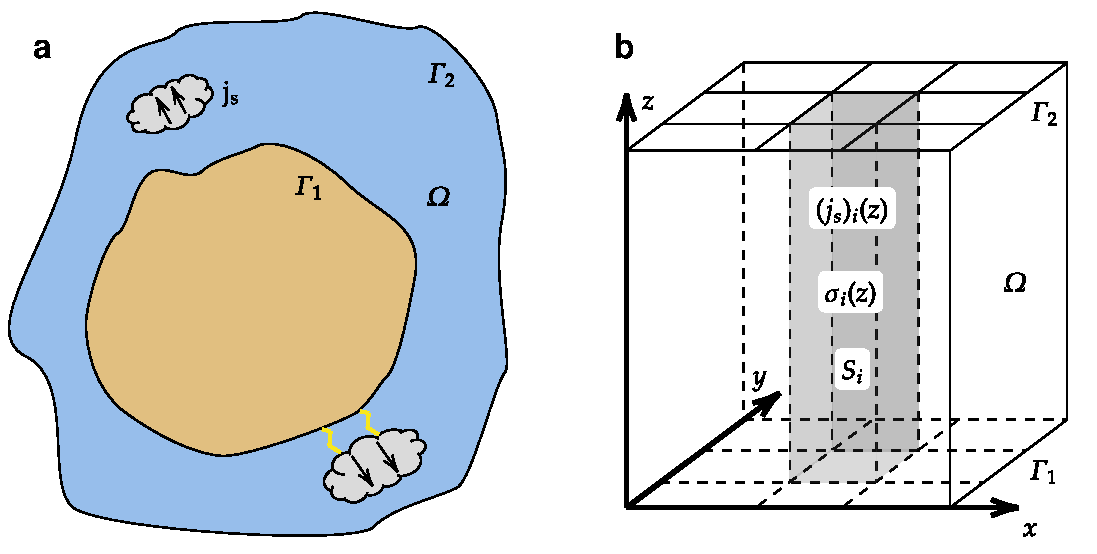
\includegraphics[width=\textwidth]{figures/gec-scheme.pdf}
    \caption{(a): Схематичное изображение ГЭЦ. (b): Иллюстрация к столбчатой модели ГЭЦ.}
    \label{fig:gec-scheme}
\end{figure}

Важно заметить, что проводимость Земли превышает проводимость приповерхностного воздуха на несколько порядков \cite[Рис. 1]{Mareev_2010}, что позволяет положить поверхность Земли $\Gamma_1$ идеально проводящей. Кроме того, следует отметить, что проводимость воздуха экспоненциально увеличивается с высотой \cite[Рис. 1]{Mareev_2010}, что позволяет считать и поверхность $\Gamma_2$ идеально проводящей, если она достаточно удалена от $\Gamma_1$ (так далеко, чтобы проводимость воздуха достигла величин, сопоставимых с проводимостью поверхности Земли, обычно это $\sim 70\, \textnormal{км}$). Такие рассуждения приводят к граничным условиям на тангенциальную компоненту электрического поля
\begin{equation}
    E_\tau \eval_{\Gamma_1} = 0,\; E_\tau \eval_{\Gamma_2} = 0.
    \label{eq:gu_pol}
\end{equation}

Таким образом, уравнения \eqref{eq:5} и \eqref{eq:6} c граничными условиями \eqref{eq:gu_pol} позволяют по заданным источникам $\vb{j}_s(\vb{r})$ и проводимости $\sigma(\vb{r})$ найти поля $\vb{E}(\vb{r})$ и $\curl{\vb{H}(\vb{r})}$.

\subsubsection{ФОРМУЛИРОВКА ЗАДАЧИ В ТЕРМИНАХ ПОТЕНЦИАЛА}

Из уравнения \eqref{eq:6} следует возможность введения потенциала, то есть такой функции $\varphi(\vb{r})$, что 
\begin{equation}
    \vb{E} = - \grad{\varphi}.
    \label{eq:11}
\end{equation}
Граничные условия \eqref{eq:gu_pol} для потенциала $\varphi(\vb{r})$ можно переписать в виде
\begin{equation}
    \varphi\eval_{\Gamma_1} = 0,\; \varphi\eval_{\Gamma_1} = V,
    \label{eq:gu_pot}
\end{equation}
где $V=\mathrm{const}$ --- ионосферный потенциал, который полагается неизвестной константой и находится в ходе решения задачи.

На потенциал $\varphi(\vb{r})$ можно записать следующую систему уравнений:
\begin{equation}
    \div{\qty(- \sigma \grad{\varphi} + \vb{j}_s)} = 0,
    \label{eq:13}
\end{equation}
\begin{equation}
    \oint\limits_{\Gamma_1} \qty(- \sigma \grad{\varphi} + \vb{j}_s) \dd{\vb{s}} = 0.
    \label{eq:14}
\end{equation}
Такие уравнения вместе эквивалентны уравнению \eqref{eq:5}. Действительно, векторное поле $\vb{X}$ может быть записано в виде ротора некоторого поля $\vb{Y}$ в области $\Omega$ тогда и только тогда, когда одновременно выполняется два условия: $\div{\vb{X}} = 0$ и равен нулю поток поля $\vb{X}$ через поверхность $\Gamma_1$ или $\Gamma_2$. При этом поле $\vb{Y}$ получается неопределенным с точностью до градиента некоторой функции $\chi$%, то есть всегда можно подобрать такое $\chi$, чтобы занулить $\div{\vb{Y}}$.
. Если возвращаться от общих рассуждений к конкретике, то в настоящем случае роль $\vb{X}$ играет векторное поле $- \sigma \grad{\varphi} + \vb{j}_s$, а роль $\vb{Y}$ --- напряженность магнитного поля $\vb{H}$, как видно из \eqref{eq:5}. Важно заметить, что уравнения \eqref{eq:13} и \eqref{eq:14} не только эквивалентны уравнению \eqref{eq:5}, но и не противоречат уравнению \eqref{eq:7} (которому можно удовлетворить, пользуясь тем, что $\vb{H}$ получается неопределенным с точностью до градиента некоторой функции $\chi$, которую всегда можно выбрать таким образом, чтобы удовлетворить \eqref{eq:7}).

Таким образом, для нахождения потенциала электрического поля $\varphi(\vb{r})$ при заданных источниках $\vb{j}_s(\vb{r})$ и проводимости $\sigma(\vb{r})$ требуется решить уравнения \eqref{eq:13} и \eqref{eq:14} с граничным условием \eqref{eq:gu_pot}. Корректность такой задачи обсуждается в \cite{Kalinin_et_al_2014}.

\subsubsection{ФОРМУЛИРОВКА ЗАДАЧИ НА ПОТЕНЦИАЛ В РАМКАХ СТОЛБЧАТОЙ МОДЕЛИ}
\label{sec:stolb}

В рамках столбчатой модели ГЭЦ поверхности $\Gamma_1$ и $\Gamma_2$ полагаются плоскостями, расположенными ортогонально оси высот $z$ (см. рис. \ref{fig:gec-scheme}{b}; обоснованность такого подхода будет обсуждена ниже в разделе \ref{sec:obosn}), при этом можно считать, что ось $x$, например, долготам, а ось $y$ --- широтам. Поверхностям $\Gamma_1$ и $\Gamma_2$ соответствуют высоты $z=0$ и $z=H_0$. Область атмосферы $\Omega$, которая теперь имеет форму прямоугольного параллелепипеда, разбивается на не перекрывающиеся цилиндры (столбцы) с образующими, параллельными оси высот $z$. В каждом столбце потенциал $\varphi(\vb{r})$ полагается изменяющимся лишь вдоль оси высот $z$, то есть $\pdv*{\varphi}{x} = \pdv*{\varphi}{y} = 0$ внутри каждого отдельного столбца. Таким образом, если в исходной постановке задачи потенциал $\varphi(\vb{r})$ был непрерывной функцией точки в области $\Omega$, то при переходе к столбчатой модели сохраняется лишь непрерывная зависимость потенциала от высоты $z$, а зависимость от поперечных координат дискретизируется и переходит в зависимость потенциала от номера столбца.

В рамках рассматриваемого приближения уравнения \eqref{eq:13} и \eqref{eq:14} принимают вид
\begin{equation}
    \dv{z}\qty(\sigma_i(z)\dv{\varphi_i}{z}\qty(z) - \qty(j_\mathrm{s})_i\qty(z)) = 0,\; i=\overline{1,\, N},
    \label{eq:15}
\end{equation}
\begin{equation}
    \sum\limits_{i=1}^{N} \qty(\sigma_i(z)\dv{\varphi_i}{z}\qty(z) - \qty(j_\mathrm{s})_i\qty(z))\cdot S_i = 0,
    \label{eq:16}
\end{equation}
где $i$ --- номер столбца, $S_i$ --- площадь основания столбца, $\qty(j_\mathrm{s})_i\qty(z)$ --- проекция тока источников в $i$-ом столбце на ось высот $z$. Следует заметить, что уравнение \eqref{eq:13} переходит в уравнение \eqref{eq:15} в рамках столбчатой модели, только если пренебречь поперечными токами, то есть $(\vb{j}_\mathrm{s})_{\perp} = 0$. Такое приближение хорошо работает в ГЭЦ из-за значительной разнице в двух пространственных масштабах: поперечный размер ГЭЦ сильно больше вертикального (поэтому токи в основном текут вдоль вертикали, по пути наименьшего сопротивления). Уравнение \eqref{eq:15} означает постоянство величины $\sigma_i(z)\dv*{\varphi_i}{z}\qty(z) - \qty(j_\mathrm{s})_i\qty(z)$ внутри $i$-ого столбца, что в свою очередь позволяет распространить \eqref{eq:14} с $\Gamma_1$ на любую поверхность между $\Gamma_1$ и $\Gamma_2$ и получить \eqref{eq:16}. Граничные же условия \eqref{eq:gu_pot} перейдут в следующие условия:
\begin{equation}
    \varphi_i\qty(z=0) = 0,\;  \varphi_i\qty(z=H_0) = V,\; i=\overline{1,\, N},
    \label{eq:gu_pot_stolb}
\end{equation}
где $V = \mathrm{const}$ --- ионосферный потенциал, полагаемый в ходе решения задачи неизвестной константой.

В итоге в рамках столбчатой модели ГЭЦ уравнения \eqref{eq:15} и \eqref{eq:16} с граничными условиями \eqref{eq:gu_pot_stolb} позволяют найти потенциал электрического поля $\varphi(\vb{r})$, если в каждом из $N$ столбцов модели заданы высотные профили проводимости $\sigma_i\qty(z)$ и плотности тока источников $\qty(j_\mathrm{s})_i\qty(z)$, а так же площади оснований $S_i$.

\subsubsection{АНАЛИТИЧЕСКОЕ РЕШЕНИЕ ЗАДАЧИ В РАМКАХ СТОЛБЧАТОЙ МОДЕЛИ}

Для решения задачи удобно ввести ток
\begin{equation}
    I_i (z) = \qty(\qty(j_\mathrm{s})_i\qty(z) - \sigma_i(z)\dv{\varphi_i}{z}\qty(z)) \cdot S_i,\; i=\overline{1,\, N}.
    \label{eq:I_i}
\end{equation}
Важно заметить, что из уравнения \eqref{eq:15} следует, что величины $I_i$ не зависят от высоты $z$ и являются постоянными для каждого отдельного столбца модели. 

Из определения \eqref{eq:I_i} можно выразить 
\begin{equation}
    \dv{\varphi_i}{z}\qty(z) = \dfrac{\qty(j_\mathrm{s})_i\qty(z) - I_i / S_i}{\sigma_i(z)},\; i=\overline{1,\, N},
\end{equation}
а затем проинтегрировать по высоте $z$ от $z=0$ до $z=z'$, что приведет к соотношению
\begin{equation}
    \varphi_i(z)\eval_{0}^{z'} = \int\limits_{0}^{z'} \dfrac{(j_\mathrm{s})_i}{\sigma_i} \dd{z} - \dfrac{I_i}{S_i} \int\limits_{0}^{z'} \dfrac{1}{\sigma_i} \dd{z}.
    \label{eq:phi}
\end{equation}
Если в качестве верхнего предела интегрирования положить высоту второй поверхности $\Gamma_2$, то есть $z'=H_0$, то из \eqref{eq:phi} получается выражение ИП
\begin{equation}
    V = \varphi_i(z)\eval_{0}^{H_0} = \int\limits_{0}^{H_0} \dfrac{(j_\mathrm{s})_i}{\sigma_i} \dd{z} - \dfrac{I_i}{S_i} \int\limits_{0}^{H_0} \dfrac{1}{\sigma_i} \dd{z}.
    \label{eq:21}
\end{equation}
Данное выражения для ИП не является конечным, так как в нем присутствует неизвестная величина $I_i$, ее следует исключить. Для этого надо воспользоваться уравнением \eqref{eq:16}, которое равноценно условию $\sum_{i=1}^N I_i = 0$. Если выразить из \eqref{eq:21} ток $I_i$ и просуммировать получившееся выражение по всем $i$, то удастся прийти к следующему выражению для ИП:
\begin{equation}
    V = \sum\limits^N_{i=1}\qty(S_i \int\limits_0^{H_0} \dfrac{(j_\mathrm{s})_i}{\sigma_i} \dd{z} \Bigg/
    \int\limits_0^{H_0} \dfrac{\dd{z}}{\sigma_i})
    \Bigg/
    \sum\limits^N_{i=1}\qty( S_i \Bigg/ {\int\limits_0^{H_0} \dfrac{\dd{z}}{\sigma_i}}).
    \label{eq:ip_stolb}
\end{equation}

Кроме того, возможно получить выражение и на высотный профиль потенциала $\varphi_i(z)$. Для этого следует подставить в \eqref{eq:phi} граничное условие на $\Gamma_1$ и выражение для $I_i$ через ИП, которое возможно получить из \eqref{eq:21}. Тогда не трудно видеть, что высотный профиль потенциала будет даваться выражением
\begin{equation}
    \varphi_i (z) = \int\limits_{0}^{z} \dfrac{(j_\mathrm{s})_i}{\sigma_i} \dd{z} - \qty[\int\limits_{0}^{z} \dfrac{\dd{z}}{\sigma_i} \Bigg/ \int\limits_{0}^{H_0} \dfrac{\dd{z}}{\sigma_i}]\times \qty(\int\limits_{0}^{H_0} \dfrac{(j_\mathrm{s})_i}{\sigma_i} \dd{z} - V),
    \label{eq:phi_stolb}
\end{equation}
где ионосферный потенциал $V$ определяется из формулы \eqref{eq:ip_stolb}. Отсюда можно получить выражение для ГП в регионе хорошей погоды. Для этого следует заметить, что под регионом хорошей погоды понимается столбец без источников, то есть $(j_\mathrm{s})_i=0$ в данном столбце. Тогда дифференцирование по высоте выражения \eqref{eq:phi_stolb} дает следующее выражение для приповерхностного ГП в регионе хорошей погоды:
\begin{equation}
\label{eq:pg_ip}
    \pdv{\varphi_i}{z} \qty(z=0) = \dfrac{V}{\sigma_i(z=0)} \qty(\int\limits_{0}^{H_0} \dfrac{\dd{z}}{\sigma_i(z)})^{-1}.
\end{equation}
Данное соотношение связывает ИП и приповерхностный ГП, измеренный в хорошую погоду.

Таким образом решается задача на потенциал электрического поля в рамках столбчатой модели ГЭЦ. Формулы \eqref{eq:ip_stolb} и \eqref{eq:phi_stolb} позволяют по заданным проводимости, плотности тока источников и площадям оснований столбцов найти ИП и профиль потенциала в каждом из столбцов.

\subsubsection{ОБОСНОВАННОСТЬ ИСПОЛЬЗОВАНИЯ СТОЛБЧАТОЙ МОДЕЛИ}
\label{sec:obosn}
% В данном разделе будет рассмотрен вопрос о том, насколько обоснованны предположения, на которых строится столбцовая модель ГЭЦ. 

% привести формулу для ИП, полученную в рамках сферической модели и сравнить ее с той, что получилась в рамках столбчатой модели. Прийти к выводу, что формулы различаются незначительно.

В рамках столбчатой модели ГЭЦ атмосфера описывается как набор параллельных не перекрывающихся столбцов, внутри которых токи полагаются текущими строго вдоль вертикали, что безусловно является идеализацией. Пренебречь поперечной структурой токов можно из-за того, что поперечный масштаб ГЭЦ значительно превышает ее характерный вертикальный масштаб, а токи в основном текут вдоль пути наименьшего сопротивления --- вдоль нормали между двумя эквипотенциальными плоскостями.

Ниже будет обоснован переход от сложной формы поверхности Земли к плоской геометрии. Стандартным приближением при исследовании Земли является аппроксимация формы поверхности Земли сферой, следовательно, логично положить поверхности $\Gamma_1$ и $\Gamma_2$ сферами с радиусами $R_E = 6371\,\textnormal{км}$ и $R_E + H_0$, где $R_E$ --- радиус Земли, $H_0$ --- характерная высота нижней ионосферы, ее выбор не так критичен, если нет цели исследовать эффекты, связанные с ионосферой. Главное, чтобы поверхность $\Gamma_2$ была значительно удалена по высоте от области источников. Можно выбирать в качестве $H_0$ высоту, где проводимость воздуха становится анизотропной, то есть можно полагать $H_0 = 70\, \textnormal{км}$  \cite[Рис. 1]{Mareev_2010}.

В сферической геометрии (по аналогии со столбчатой моделью) можно устроить разбиение области $\Omega$ на маленькие области, вырезаемые в области $\Omega$ телесными углами, вершины которых расположены в центре Земли. Ниже такие маленькие области будут называться конусами. Примерный вид такого конуса представлен на рис. \ref{fig:konus}.

\begin{figure}[htbp]
    \centering
    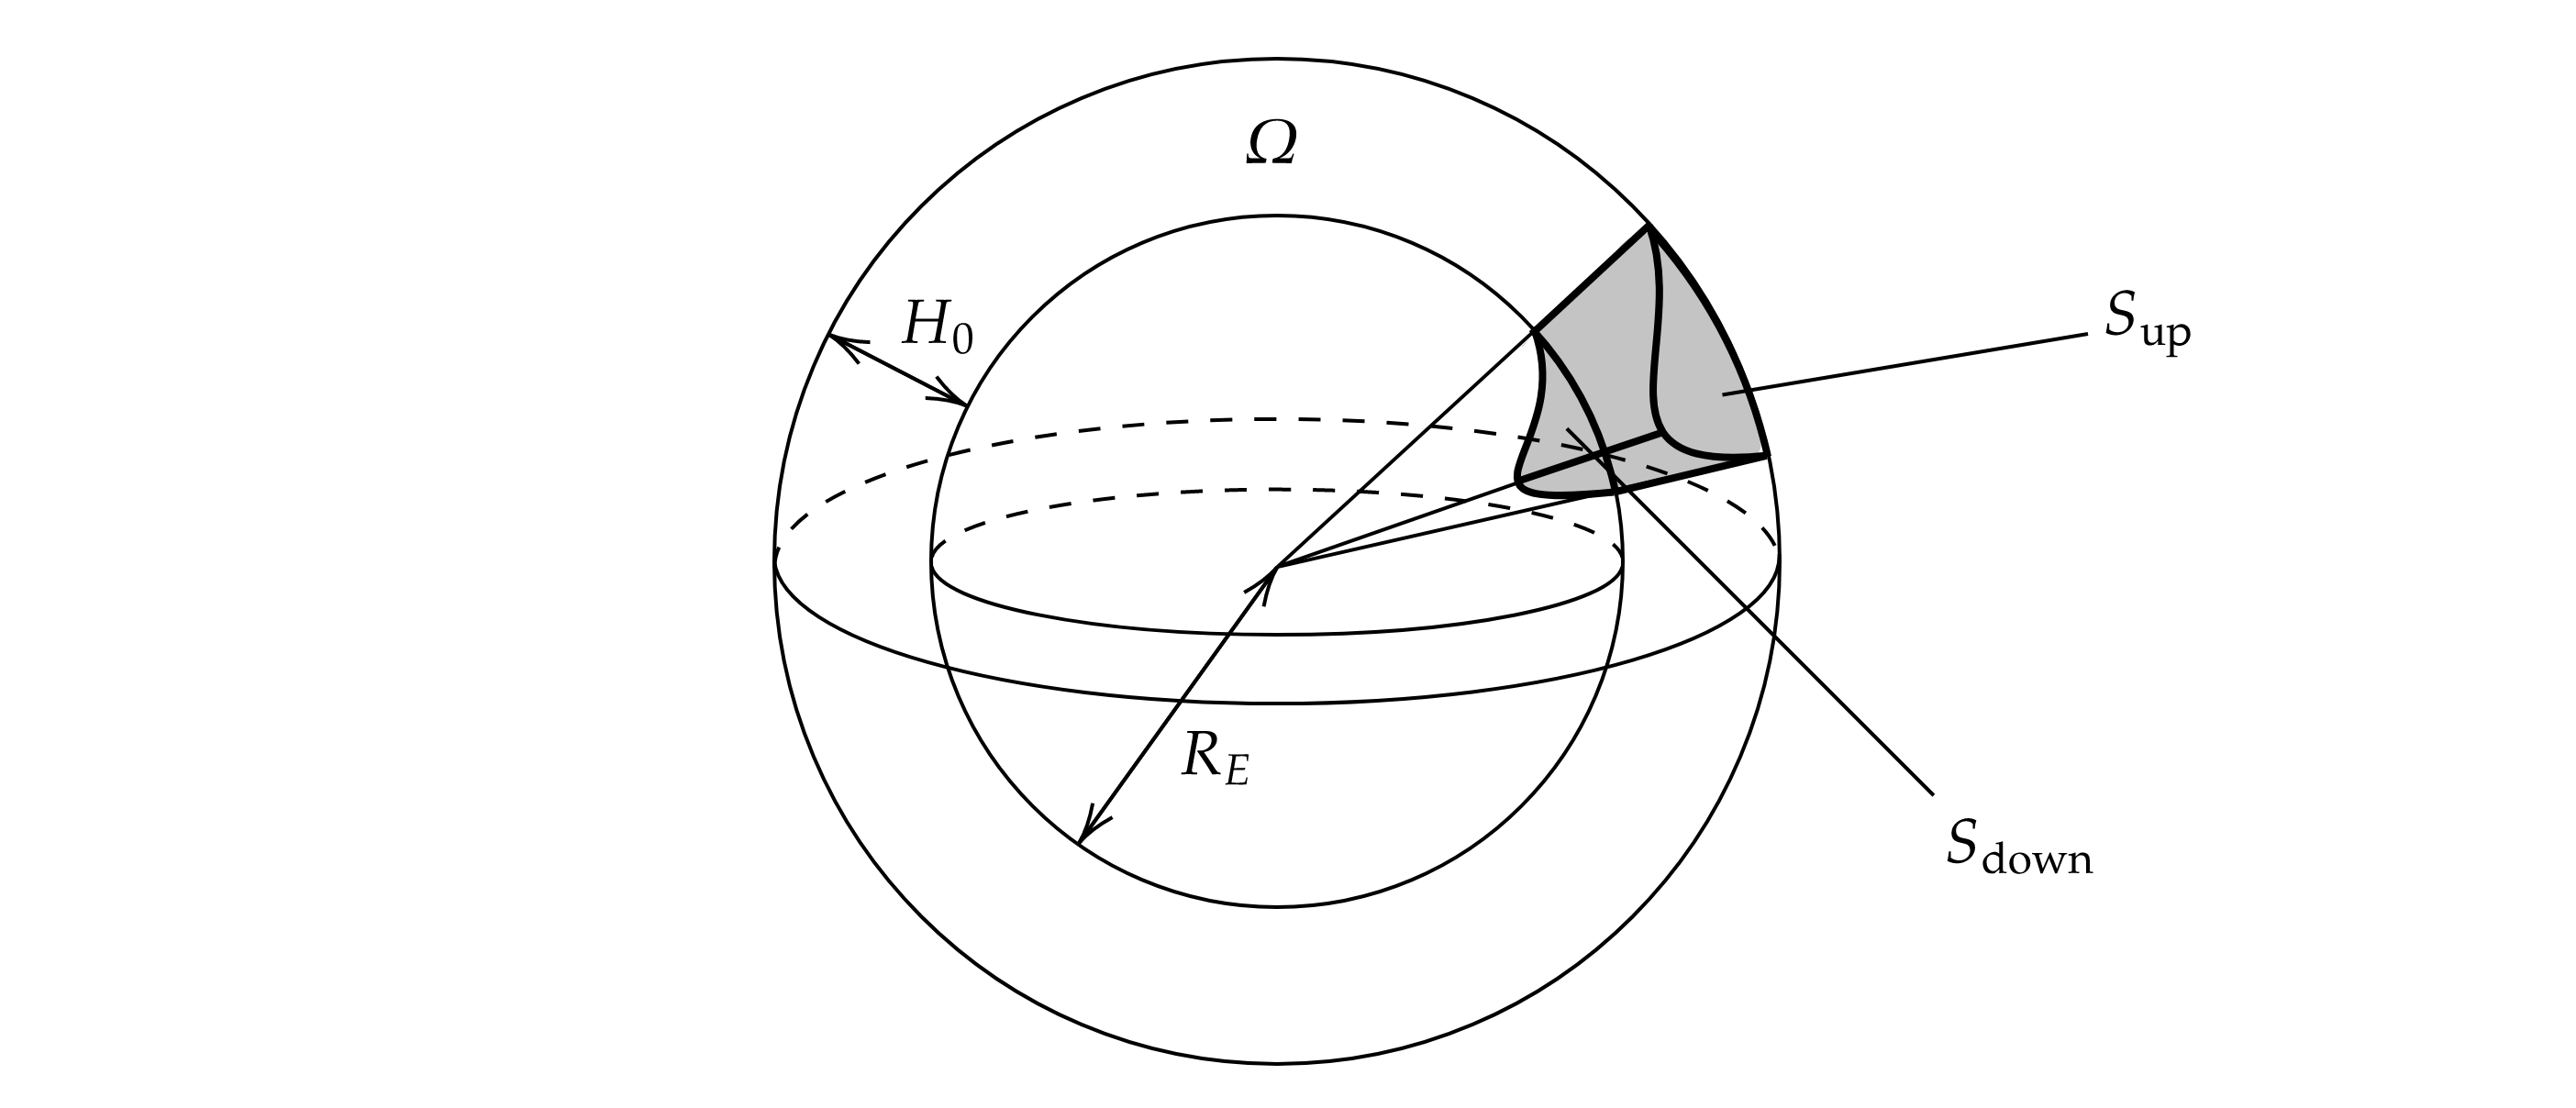
\includegraphics[width=\textwidth]{figures/konus.png}
    \caption{Примерный вид одной из маленьких областей (выделено серым), на которые разбивается область $\Omega$ в приближении сферических поверхностей $\Gamma_1$ и $\Gamma_2$.}
    \label{fig:konus}
\end{figure}

Следует заметить, что все различие между рассматриваемой моделью и столбчатой моделью сводится к различию в формах областей, на которые разбивается область $\Omega$: в данном случае это конусы, в случае столбчатой модели --- цилиндры. Главное отличие между конусами и цилиндрами заключается в том, что у первых площади верхнего и нижнего оснований различны, а у последних --- одинаковы. Для оценки того, на сколько сильно конусы отличаются от цилиндров, следует сравнить площади оснований
\begin{equation}
    \dfrac{S_\textnormal{up}}{S_\textnormal{down}} = \dfrac{\qty(R_E + H_0)^2}{R_E^2} = \qty(1 + \dfrac{H_0}{R_E})^2.
\end{equation}
Для продвижения рассуждений следует учесть, что $H_0 = 70\, \textnormal{км}$, тогда получается следующая оценка:
\begin{equation}
    \dfrac{S_\textnormal{up}}{S_\textnormal{down}} = \qty(1 + \dfrac{70}{6371})^2 \approx 1 + 2 \cdot \dfrac{70}{6371} = 1 + 2 \cdot 0.01.
\end{equation}
Отсюда следует, что такие конусы с точностью до 2\% можно полагать цилиндрами. Это доказывает справедливость рассмотрения столбчатой модели, где вместо конусов используются цилиндры.
    \subsection{РЕАЛИЗАЦИЯ СТОЛБЧАТОЙ МОДЕЛИ}

В рамках столбчатой модели получается достаточно простое выражение для ИП \eqref{eq:ip_stolb}, однако возникают трудности при задании источников и проводимости, виной чему малое количество наблюдательных данных и их противоречивость. Ниже будут описаны параметризации источников и проводимости атмосферы, которые были использованы в данной работе.

\subsubsection{ПАРАМЕТРИЗАЦИЯ ИСТОЧНИКОВ ГЭЦ}
\label{sec:sources}

В данной работе будет использована параметризация плотности тока источников, которая подробно обсуждалась в \cite{Ilin_et_al_2020}. Следует заметить, что рассматриваемая параметризация строится на результатах моделирования атмосферной динамики с помощью модели Weather Research and Forecasting (WRF) на широтно-долготной сетке 1\textdegree\texttimes1\textdegree. Ячейки такой сетки служат основаниями для столбцов модели ГЭЦ. То есть разрешение по широте и долготе, на котором придется в дальнейшем работать, составляет порядка $100\, \textnormal{км}$ вдоль долготы и вдоль широты.

Не каждый столбец содержит в себе источник. Источники есть лишь в столбцах, где присутствуют облака с развитой электрической структурой, для формирования которых нужна достаточно сильная конвекция. Поэтому появляется критерий, согласно которому во всех столбцах с максимальным по высотному профилю значением доступной конвективной потенциальной энергии (в англоязычной литературе часто используют термин convective available potential energy или CAPE) меньше порогового значения $\varepsilon_0 = 1000\, \text{Дж}/ \text{кг}$ нет токовых источников.

Далее следует заметить, что если в столбце и есть облака с развитой электрической структурой, то они не покрывают всей площади основания столбца, так как размер оснований, как отмечалось выше, крайне велик. Поэтому вводят некий коэффициент, который отражает то, какая часть площади основания столбца покрыта облаками, вносящими вклад в ГЭЦ. Таким коэффициентом выступает отношение $\alpha_i \propto P_i/W_i$ \cite{Mareev_Volodin_2014}, где $W_i$ --- количество воды, которое может выпасть в виде осадков в данном столбце, а $P_i$ --- количество выпавших осадков, посчитанное за симметричный двух-часовой интервал. Коэффициент пропорциональности обычно не важен и переносится в константу $j_0$ (см. формулу \eqref{eq:ip}).То есть площадь основания столбца разбивается на площадь области, свободной от источников, и на площадь области, ими занятую:
\begin{equation}
	S_i = S^\text{без ист.}_i + S^\text{ист.}_i,\; S^\text{ист.}_i = \alpha_i S_i.
\end{equation}
Только в части столбца над площадью $S^\text{ист.}_i$ ток источников отличен от нуля.

Осталось определить высотный профиль плотности токов источников, который для простоты задается П-образной функцией
\begin{equation}
	(j_s)_i(z) = 
	\begin{cases}
		j_0, &\text{ если }z\in\qty(z^1_i,z^2_i);\\
		0, &\text{ если }z\ \overline{\in}\ \qty(z^1_i,z^2_i);
	\end{cases}
\end{equation}
где $j_0$ --- характерная величина тока разделения зарядов в облаках с развитой электрической структурой, а через $z^1_i$ и $z^2_i$ обозначены высоты изотерм, соответствующих $0^\circ\text{C}$ и $-38^\circ\text{C}$. Такие высоты показывают характерные границы области смешанной фазы.

\subsubsection{ПРОВОДИМОСТЬ ВОЗДУХА, ЗАВИСЯЩАЯ ЛИШЬ ОТ ВЫСОТЫ}
\label{sec:exp_sigma}

Зачастую в качестве проводимости воздуха используют крайне простую функцию, которая зависит лишь от высоты, и имеет вид:
\begin{equation}
    \sigma(z) = \sigma_0 \exp\qty(z/H),
    \label{eq:cond}
\end{equation}
где $\sigma_0$ --- приповерхностное значение проводимости воздуха, а через $H$ обозначен характерный масштаб увеличения проводимости; обычно полагают $H = 6\, \textnormal{км}$. Тогда, подставляя параметризацию источников, описанную в разделе \ref{sec:sources}, и функцию проводимости \eqref{eq:cond} в выражения для ИП \eqref{eq:ip_stolb}, можно прийти к следующей формуле для ИП:
\begin{equation}\label{eq:ip}
 	V = \dfrac{j_0H}{\sigma_0 S_E} \sum\limits_i \qty[\exp\qty(-\dfrac{z^1_i}{H}) - \exp\qty(-\dfrac{z^2_i}{H})] \times \dfrac{P_i S_i}{W_i} \times \theta(\varepsilon_i - \varepsilon_0),
\end{equation}
где $S_E$ --- площадь поверхности Земли,  $\varepsilon_i$ --- максимальное значение CAPE в столбце, а под функцией $\theta(x)$ понимается функция Хевисайда. Сумма (\ref{eq:ip}) берется по всем столбцам модели. Слагаемые данной суммы принято называть вкладами в ИП. Более глубокий анализ данной формулы производится в \cite{Ilin_et_al_2020}. Важно повторить основные идеи данной параметризации: второй множитель в формуле (\ref{eq:ip}) оценивает площадь, занимаемую облаками в каждой из ячеек модели, а третий множитель позволяет выделить столбцы с развитой конвективной активностью по критерию, основанному на значении CAPE. Для расчета ИП необходимо задать параметры (высоты изотерм, осадки и CAPE), которые берутся из результатов воспроизведения атмосферной динамики.

\subsubsection{ПРОВОДИМОСТЬ ВОЗДУХА, ЗАВИСЯЩАЯ ОТ СОЛНЕЧНОЙ АКТИВНОСТИ}
\label{sec:complicated_sigma}

В данном разделе будет рассмотрена более сложная параметризация проводимости, основанная на ряде экспериментальных измерений и подробно обсуждаемая в \cite{Slyunyaev_et_al_2015}. Главной особенностью данной параметризации проводимости воздуха является учет зависимости проводимости от солнечной активности, которая модулирует поток галактических космических лучей, сильно влияющих на процессы ионизации и рекомбинации в атмосфере. Такую параметризацию проводимости не удается записать компактно, поэтому запись данной проводимости с помощью формул будет опущена в настоящей работе. В рамках данной параметризации проводимость зависит от высоты $z$, геомагнитной широты $\lambda$ и параметра $\xi\in[0,\, 1]$, характеризующего уровень солнечной активности. $\xi=0$ соответствует минимуму солнечной активности, $\xi=1$ --- максимуму. Геомагнитные координаты зависят от положений магнитных полюсов, положение которых со временем меняется; кроме того, со временем меняется и уровень солнечной активности, поэтому проводимость в рамках данной параметризации зависит и от времени, хоть и неявно.

Если рассматривать параметризацию источников, описанную в разделе \ref{sec:sources}, то выражение для ИП \eqref{eq:ip_stolb} примет вид
\begin{equation}
    V = \sum\limits^N_{i=1}j_0\qty(\dfrac{P_i S_i}{W_i} \times \theta(\varepsilon_i - \varepsilon_0) \times \int\limits_{z_i^1}^{z_i^2} \dfrac{
    \dd{z}}{\sigma_i} \Bigg/
    \int\limits_0^{H_0} \dfrac{\dd{z}}{\sigma_i})
    \Bigg/
    \sum\limits^N_{i=1}\qty( S_i \Bigg/ {\int\limits_0^{H_0} \dfrac{\dd{z}}{\sigma_i}}).
    \label{eq:ip_stolb_1}
\end{equation}
Таким образом, сосчитать ИП в рамках столбчатой модели ГЭЦ с реалистичной проводимостью, учитывающей влияние солнечной активности, возможно лишь путем численного интегрирования обратной проводимости; кроме того, как и в случае с экспоненциальной проводимостью, для расчета ИП нужны результаты воспроизведения атмосферной динамики (CAPE, данные по осадкам, запасенной влаге и высотам изотерм).





% возьми ход мысли из статьи Slyunayev_et_al_2019, оттуда описание моделирования WRF
% передай логику моделирования, сначала моделирования атмосферной динамики, откуда берутся источники, далее откуда была взята проводимость (1 абзац про проводимость), потом это все подставляется в формулу и численно интегрируется, и получается ИП и высотный профиль электрического потенциала

% следующий подраздел будет про сравнение моделей с двумя разными проводимостями, перенеси описание той модели сюда, только аккуратно



    \subsection{РЕЗУЛЬТАТЫ МОДЕЛИРОВАНИЯ}

На языке программирования C++ была реализована столбчатая модель ГЭЦ, которая позволяет рассчитывать ИП при любом задании токов источников и проводимости воздуха. Так как параметризация источников, описанная в разделе \ref{sec:sources}, имеет ясный физический смысл, то ниже всюду будет использоваться именно она.

ИП и электрическое поле в регионах хорошей погоды имеют замечательную особенность --- устойчивую кривую суточной вариации. Такую кривую называют кривой Карнеги \cite{Harrison_2012} (см. рис. \ref{fig:carnegie_curve}). Ее форма объясняется динамикой глобальных грозовых центров, происходящей на масштабах суток \cite{Ilin_et_al_2020}. Кривая Карнеги служит хорошим объектом для проверки адекватности работы реализованной столбчатой модели ГЭЦ. 

\begin{figure}  
    \centering
    \begin{subfigure}[t]{.49\textwidth}
		\centering
		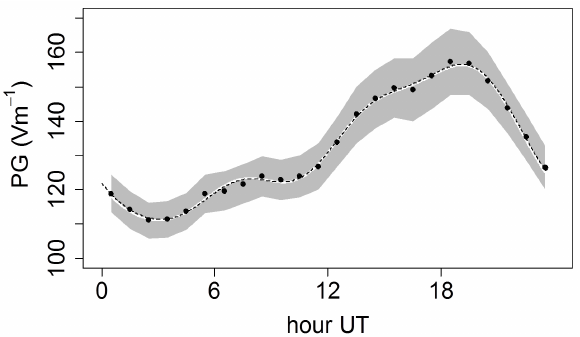
\includegraphics[width=\linewidth]{figures/carnegie_curve.png}
		\caption{}
		\label{fig:carnegie_curve}  
    \end{subfigure}
    \hfill
    \begin{subfigure}[t]{.49\textwidth}
		\centering
		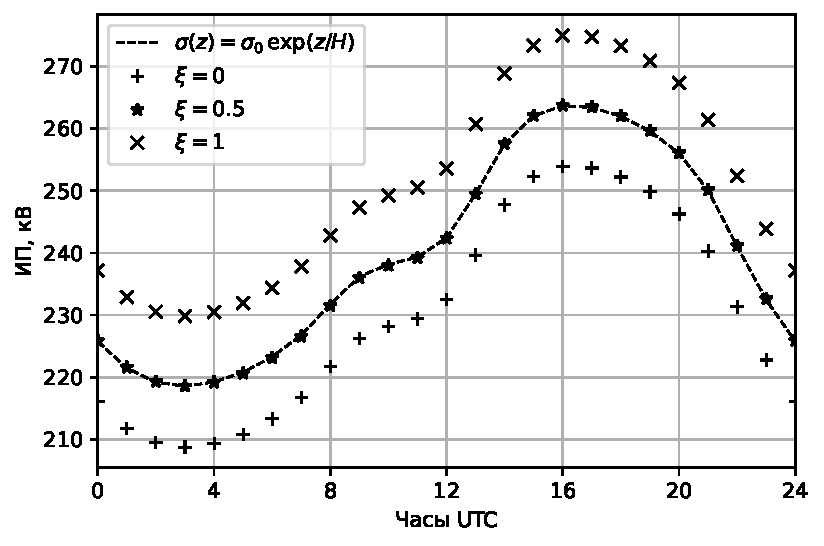
\includegraphics[width=\linewidth]{figures/ip_differences.pdf}
		\caption{}
		\label{fig:ip_differences}  
     \end{subfigure}
     \caption{(a): Черные точки изображают вариацию приповерхностного градиента потенциала электрического поля (potential gradient, PG) по часам всемирного времени (UTC), измеренную на корабле Карнеги в 1920-ые годы. Серая область вокруг точек обозначает плюс и минус одну стандартную ошибку среднего. Черная пунктирная и белая линии обозначают различные гладкие аппроксимации экспериментальных данных. Взято из \cite[Рис. 6a]{Harrison_2012} (b): Пунктирной линией обозначена кривая суточной вариации ИП, полученная при усреднении результатов моделирования ИП с экспоненциальной проводимостью (см. раздел \ref{sec:exp_sigma}) за каждый третий день 2016 года. Суточные вариации ИП, получаемые при использовании параметризации проводимости, описанной в разделе \ref{sec:complicated_sigma}, отмечены точечными маркерами: маркер плюс отвечает моделированию при параметре $\xi$, описывающем солнечную активность, равном 0; маркер звездочка --- при $\xi = 0.5$; маркер крест --- при $\xi = 1$.}
	\label{fig:variations-1}  
\end{figure}

Параметризация источников, описанная в разделе \ref{sec:sources}, требует задания таких параметров, как высоты изотерм, осадки, запасенная влага и CAPE, которые берутся из результатов воспроизведения атмосферной динамики. Для этих целей использовалась метеорологическая модель WRF, позволившая получить требуемые для расчета ИП параметры в виде 24-часового набора данных за каждый третий день 2016 года на широтно-долготной сетке 1\textdegree\texttimes1\textdegree. На основе данных, полученных из модели WRF, рассчитывался ИП. В результате таких расчетов получался 24-часовой набор значений ИП для каждого третьего дня 2016 года.

Было произведено несколько серий расчетов ИП. В различных сериях расчетов использовались разные параметризации проводимости: в одном из расчетов была задействована параметризация проводимости, описанная в разделе \ref{sec:exp_sigma}, в прочих расчетах использовалась более сложная параметризация проводимости, которой был посвящен раздел \ref{sec:complicated_sigma}), с различными параметрами солнечной активности $\xi$. 

Результаты расчетов ИП усреднялись по всем моделируемым дням, чтобы получить кривую суточной вариации ИП (даже моделируемый ИП крайне изменчив на масштабах суток, поэтому для обнаружения характерной кривой суточной вариации необходимо усреднять данные по достаточно долгому периоду времени). В итоге были получены кривые суточной вариации ИП, изображенные на рис. \ref{fig:ip_differences}.

Из анализа полученных кривых удается сделать три вывода. Первый состоит в том, что разработанная модель ГЭЦ позволяет получать кривую суточной вариации ИП, близкую к оригинальной кривой Карнеги (как видно из сравнения рис. \ref{fig:ip_differences} с рис. \ref{fig:carnegie_curve}), что подтверждает верность реализации столбчатой модели ГЭЦ. Второй вывод заключается в том, что форма кривой суточной вариации ИП, получающаяся при моделировании с экспоненциальной проводимостью, совпадает с формой кривой суточной вариации, которая получается при моделировании с учетом более реалистичной проводимости (см. рис. \ref{fig:ip_differences}), то есть кривые имеют максимумы и минимумы в одни и те же часы UTC. В качестве третьего вывода следует отметить, что учет более реалистичной проводимости приводит к повышению ИП примерно на $10\, \textnormal{кВ}$ в фазу максимума солнечной активности и к понижению примерно на те же $10\, \textnormal{кВ}$ в фазу минимума солнечной активности по сравнению со значениями ИП, получаемыми при моделировании с экспоненциальной проводимостью.
    % вывод уравнений на потенциал
    % реализация столбцовой модели ГЭЦ ? (тут про проводимости тинсли)
    % описание модели ГЭЦ с более простой проводимостью ??
    % сравнение двух моделей и оценка нужности учёта более тонкой параметризации проводимости
    \newpage
    \section{ВЛИЯНИЕ КОЛЕБАНИЯ МАДДЕНА--ДЖУЛИАНА НА ГЛОБАЛЬНУЮ ЭЛЕКТРИЧЕСКУЮ ЦЕПЬ}
    \Subsection{ХАРАКТЕРИСТИКА КОЛЕБАНИЯ МАДДЕНА--ДЖУЛИАНА}


    \subsection{МОДЕЛИРОВАНИЕ ГЭЦ С ПРОВОДИМОСТЬЮ, ЗАВИСЯЩЕЙ ТОЛЬКО ОТ ВЫСОТЫ}

В данной части работы использовалась модель ГЭЦ, основанная на параметризации ИП с экспоненциальной проводимостью (см. раздел \ref{sec:exp_sigma}), то есть использовалась формула \eqref{eq:ip}. Для расчета ИП в рамках данной параметризации необходимо задать параметры (высоты изотерм, осадки и CAPE), которые берутся из результатов воспроизведения атмосферной динамики. Для этих целей использовалась модель WRF, позволившая получить требуемые для расчета ИП параметры в виде 24-часового набора данных за каждый третий день с 1 января 1980 года по 29 декабря 2020 года на широтно-долготной сетке 1\textdegree\texttimes1\textdegree. 

%В данной части работы использовалась модель ГЭЦ, основанная на параметризации ИП, предложенной в \cite{Slyunyaev_et_al_2019} на основе идей \cite{Mareev_Volodin_2014}.
%Такая параметризация использует функцию проводимости, которая зависит лишь от высоты $\sigma(z)  = \sigma_0 \exp\qty(z/H)$, и определяет вклады в ИП от каждой ячейки модельной сетки в терминах климатических параметров так, что ИП дается выражением
%\begin{equation}\label{eq:ip}
% 	V = \dfrac{j_0H}{\sigma_0 S_E} \sum\limits_i \qty[\exp\qty(-\dfrac{z^1_i}{H}) - %\exp\qty(-\dfrac{z^2_i}{H})] \times \dfrac{P_i S_i}{W_i} \times \theta(\varepsilon_i - \varepsilon_0),
%\end{equation}
%где $j_0$ --- характерная величина тока разделения зарядов в облаках с развитой электрической структурой, $\sigma_0$ и $H$ приповерхностное значение проводимости воздуха и характерный масштаб увеличения проводимости (в вычислениях полагается $H=6\,\textnormal{км}$), $S_i$ --- площадь, занимаемая $i$-ой ячейкой; $P_i$, $W_i$, $\varepsilon_i$, $z_i^1$ и $z_i^2$ --- общее количество осадков, взятой за симметричный двух часовой интервал, общее количество влаги, максимальное значение convective available potential energy (CAPE) и верхняя и нижняя границы области смешанной фазы в облаке (которые приближались высотами изотерм $0$ \textdegree C и $-38$ \textdegree C) в $i$-ом столбце соответственно, а $\varepsilon_0$ --- граничное значение CAPE, которое полагалось в расчетах $1\, \textnormal{кДж}/\textnormal{кг}$. Сумма (\ref{eq:ip}) берется по по всем столбцам модели. Более глубокий анализ данной формулы производится в \cite{Ilin_et_al_2020}. Важно отметить основные идеи данной параметризации: второй множитель в формуле (\ref{eq:ip}) оценивает площадь, занимаемую облаками в каждой из ячеек модели, а третий множитель позволяет выделить столбцы с развитой конвективной активностью по критерию, основанному на значении CAPE.
%
%Для расчета ИП необходимо задать параметры (высоты изотерм, осадки и CAPE), которые берутся из результатов воспроизведения атмосферной динамики. Для этих целей использовалась Weather Research and Forecasting model (WRF), позволившая получить требуемые для расчета ИП параметры в виде 24-часового набора данных за каждый третий день с 1 января 1980 года по 29 декабря 2020 года на широтно-долготной сетке 1\textdegree\texttimes1\textdegree. 
%
%В итоге были рассчитаны значения ИП за каждый третий день с 1 января 1980 года по 29 декабря 2020 (и вкладов в ИП за тот же период на на широтно-долготной сетке 1\textdegree\texttimes1\textdegree). Значение величины $j_0$ в (\ref{eq:ip}) является параметром модели, оно подбиралось таким образом, чтобы среднее значение моделируемого ИП было равно $240\,\textnormal{кВ}$, что соответствует типичному значению ИП \cite{Markson_2007}.
    \subsection{ИЗМЕРЕНИЯ ЭЛЕКТРИЧЕСКОГО ПОЛЯ НА СТАНЦИИ ВОСТОК}\label{sec:vostok}

За исключением моделирования ГЭЦ с помощью модели WRF в настоящей части работы используются результаты измерений ГП на российской антарктической станции Восток (78.5\textdegree\ ю. ш., 106.9\textdegree\ в. д., $3488\,\textnormal{м}$ над уровнем моря) за период 2006--2020. Такие измерения ГП собираются в удалённом месте и представляют уникальный длинный набор, описывающих ГЭЦ \cite{Burns_et_al_2012,Burns_et_al_2017}.

Электрическое поле измеряется с помощью датчика --- вращающегося диполя, который был установлен на станции Восток в конце 2005 года в рамках российской-австралийского соглашения \cite{Burns_et_al_2017}. Вращающийся диполь установлен на высоте $3\,\textnormal{м}$ на уровнем снежного покрова, возвышаясь над основными строениями станции. Величины ГП собираются в форме усредненных за 10-секундные интервалы значений. По техническим причинам данные имеют большой пропуск во второй половине 2017 года и несколько пропусков поменьше в иное время; кроме того, для некоторых периодов времени доступны только 5-минутные данные.

Чтобы упростить анализ, данные измерений усреднялись по часам UTC, при этом, если доступны как 10-секундные данные, так и 5-минутные данные, брались 10-секундные. При усреднении рассматривались лишь те часы, для которых было записано хотя бы 80\% 10-секундных или 5-минутных значений ГП. Все измеренные значения ГП делились на форм-фактор, равный $3$, для устранения помех, вызванных металлическим стержнем, поддерживающим датчик электрического поля.

Дни хорошей погоды выбирались на основе подхода, примененного в \cite{Slyunyaev_et_al_2021a}. Чтобы выделить дни хорошей погоды, не обязательно использовать метеорологические данные, можно воспользоваться критерием, основанным на значениях ГП, который обычно работает достаточно хорошо \cite{Burns_et_al_2012,Burns_et_al_2017}. Следующая формальная процедура применялась к наборам данных ГП:
\begin{enumerate}
	\item Исключаются дни с неполными или пропущенными часовыми значениями.
	\item Из рассмотрения убираются дни с отрицательными или нулевыми значениями ГП.
	\item Исключаются дни с часовыми значениями ГП, превышающими $300\,\textnormal{В}/\textnormal{м}$.
	\item Среди оставшихся дней удерживаются только те, в которых разница между максимумом суточной вариации и ее минимумом не превышает 150\% от среднесуточного значения.
\end{enumerate}

    \subsection{ЭФФЕКТЫ КМД В МОДЕЛИ ГЭЦ}
\label{sec:eff_mjo_gec}

Чтобы обнаружить паттерны КМД в моделируемой ГЭЦ за период 1980--2020, величины вкладов в ИП усреднялись по дням, отвечающим каждой из восьми фаз КМД. Такие фазы определяются на основе полярного угла на плоскости (RMM1, RMM2) (см. рис. \ref{fig:wh04_fig7}); в среднем в течение цикла КМД точка на данной плоскости движется по окружности вокруг начала координат против часовой стрелки, проходя все фазы. Обычно рассматривают не только фазу, но и амплитуду (расстояние от точки до начала координат), что позволяет разделять КМД на слабое и сильное (см. рис. \ref{fig:wh04_fig7}). В данной работе амплитуда индекса RMM не рассматривалась, так как не было обнаружено какой-либо зависимости в обнаруженных эффектах от нее.

Одной из главных черт КМД является перенос с запада на восток крупномасштабной конвективной структуры в тропиках. Исходя из параметризации ИП (\ref{eq:ip}), вклады в ИП от столбцов модели во многом зависят от CAPE и осадков~---~параметров, связанных с глубокой конвекцией. Поэтому разумно предположить, что паттерны КМД будут заметны во вкладах в ИП.

Так как КМД является нерегулярным процессом, то не следует рассматривать отдельные циклы КМД~---~они могут значительно отличаться друг от друга. Альтернативой такому подходу является переход к некоторому универсальному для КМД временному масштабу~---~масштабу 8 фаз, поэтому среднесуточные значения вкладов в ИП усреднялись по дням, приходящимся на каждую из фаз КМД. Затем вычиталось среднее за длительный период времени значение каждого вклада из усредненных по фазам КМД значений. Таким образом осуществлялся переход к аномалиям вкладов, которые легко интерпретировать: положительная аномалия означает, что данный столбец модели дает вклад в ИП больше, чем обычно, а отрицательная аномалия означает, что вклад данного столбца в ИП ниже обычного значения.

Рис. \ref{fig:map_of_contributions} показывает, как такие аномалии во вкладах меняются с фазой КМД. Видно, что положительная и отрицательная аномалии перемещаются с запада на восток друг за другом с ростом номера фазы КМД. Такой эффект отражает аналогичное перемещение областей усиленной и ослабленной конвективной активности в течение цикла КМД (см. рис. \ref{fig:map_of_olr_anomaly}).

\begin{figure}[tb]
	\centering
	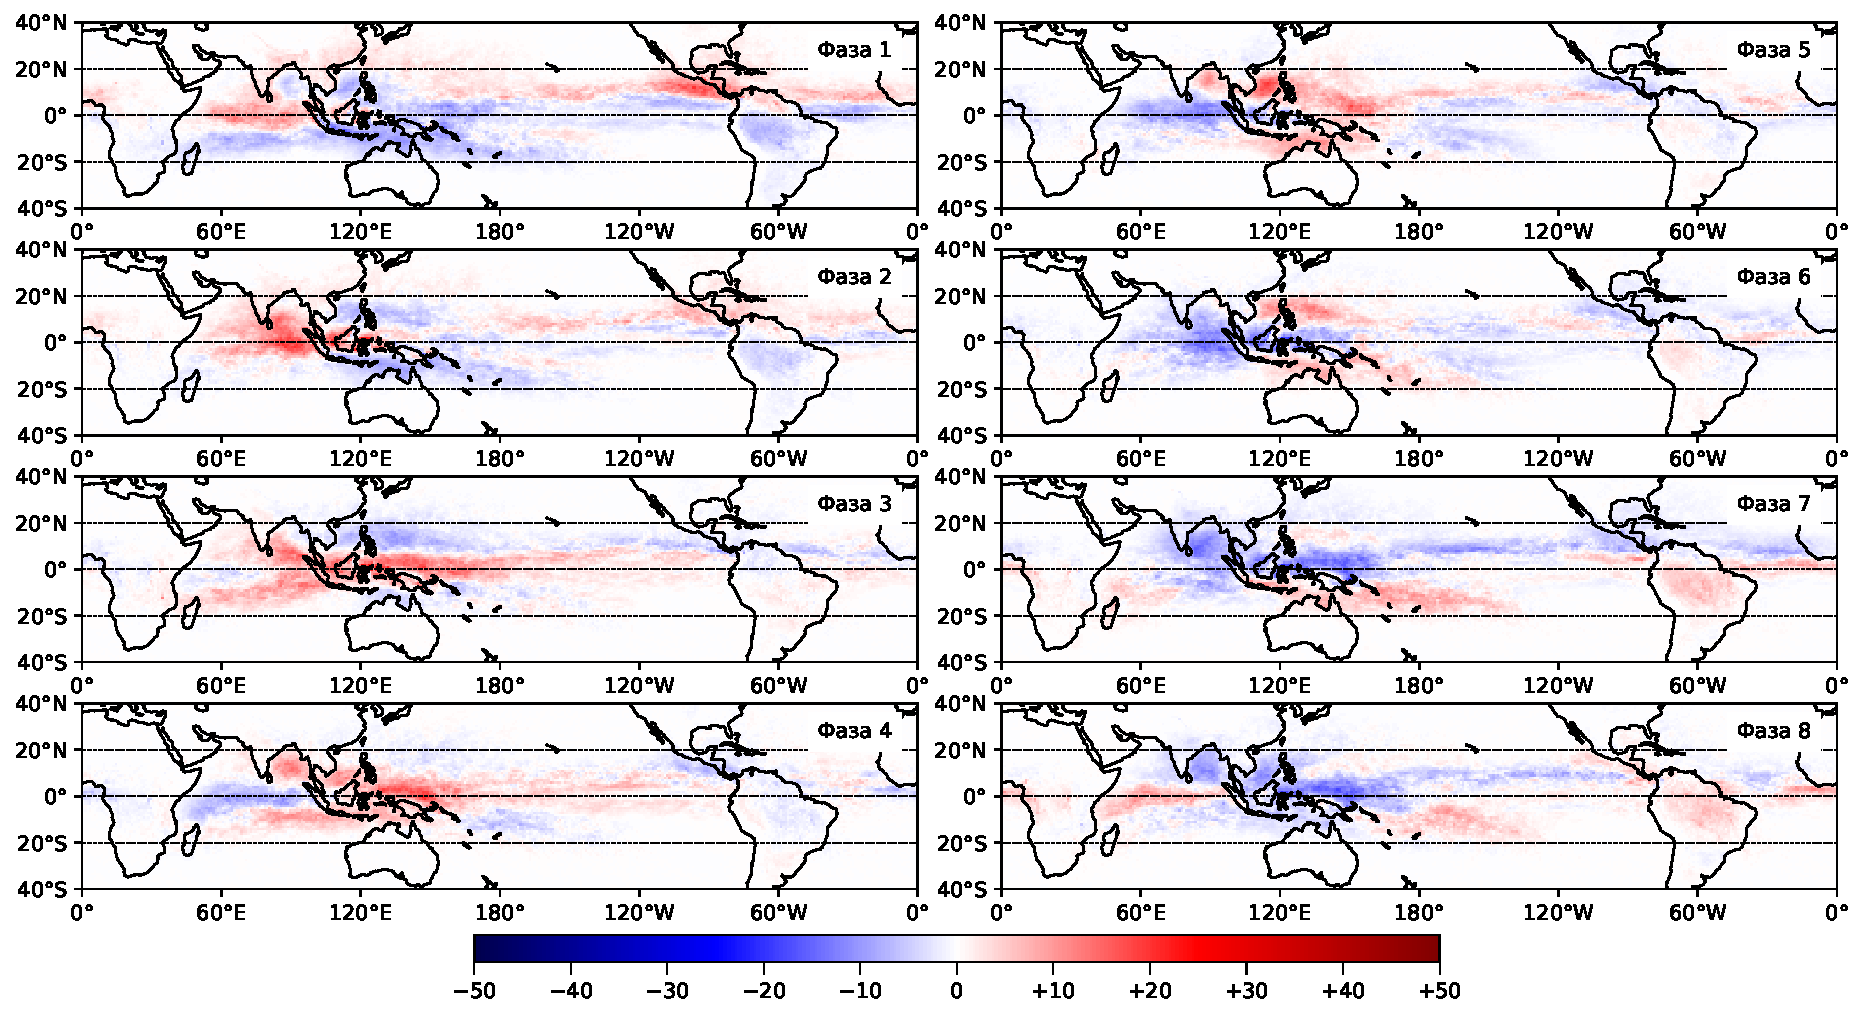
\includegraphics[width=\textwidth]{figures/map_of_contributions.pdf}
	\caption{Аномалии вкладов отдельных модельных столбцов в ИП (в вольтах) в течение каждой из фаз КМД.}
	\label{fig:map_of_contributions}
\end{figure}

Такие образом в среднем моделируемые вклады в ИП изменяются в соответствии с динамикой конвекции на масштабах КМД, что не должно быть удивительным ввиду используемой параметризации (\ref{eq:ip}). Гораздо более интересно было бы посмотреть на такой параметр модели ГЭЦ, как ИП. Рис. \ref{fig:variations}{a} показывает средние значения ИП в различные фазы КМД. Видно, что вариация имеет вид синусоиды с максимумом в фазе 3 и минимумом в фазе 7. Период синусоиды близок к восьми фазам КМД, а амплитуда составляет $12\,\textnormal{кВ}$.

\begin{figure} 
    \centering
    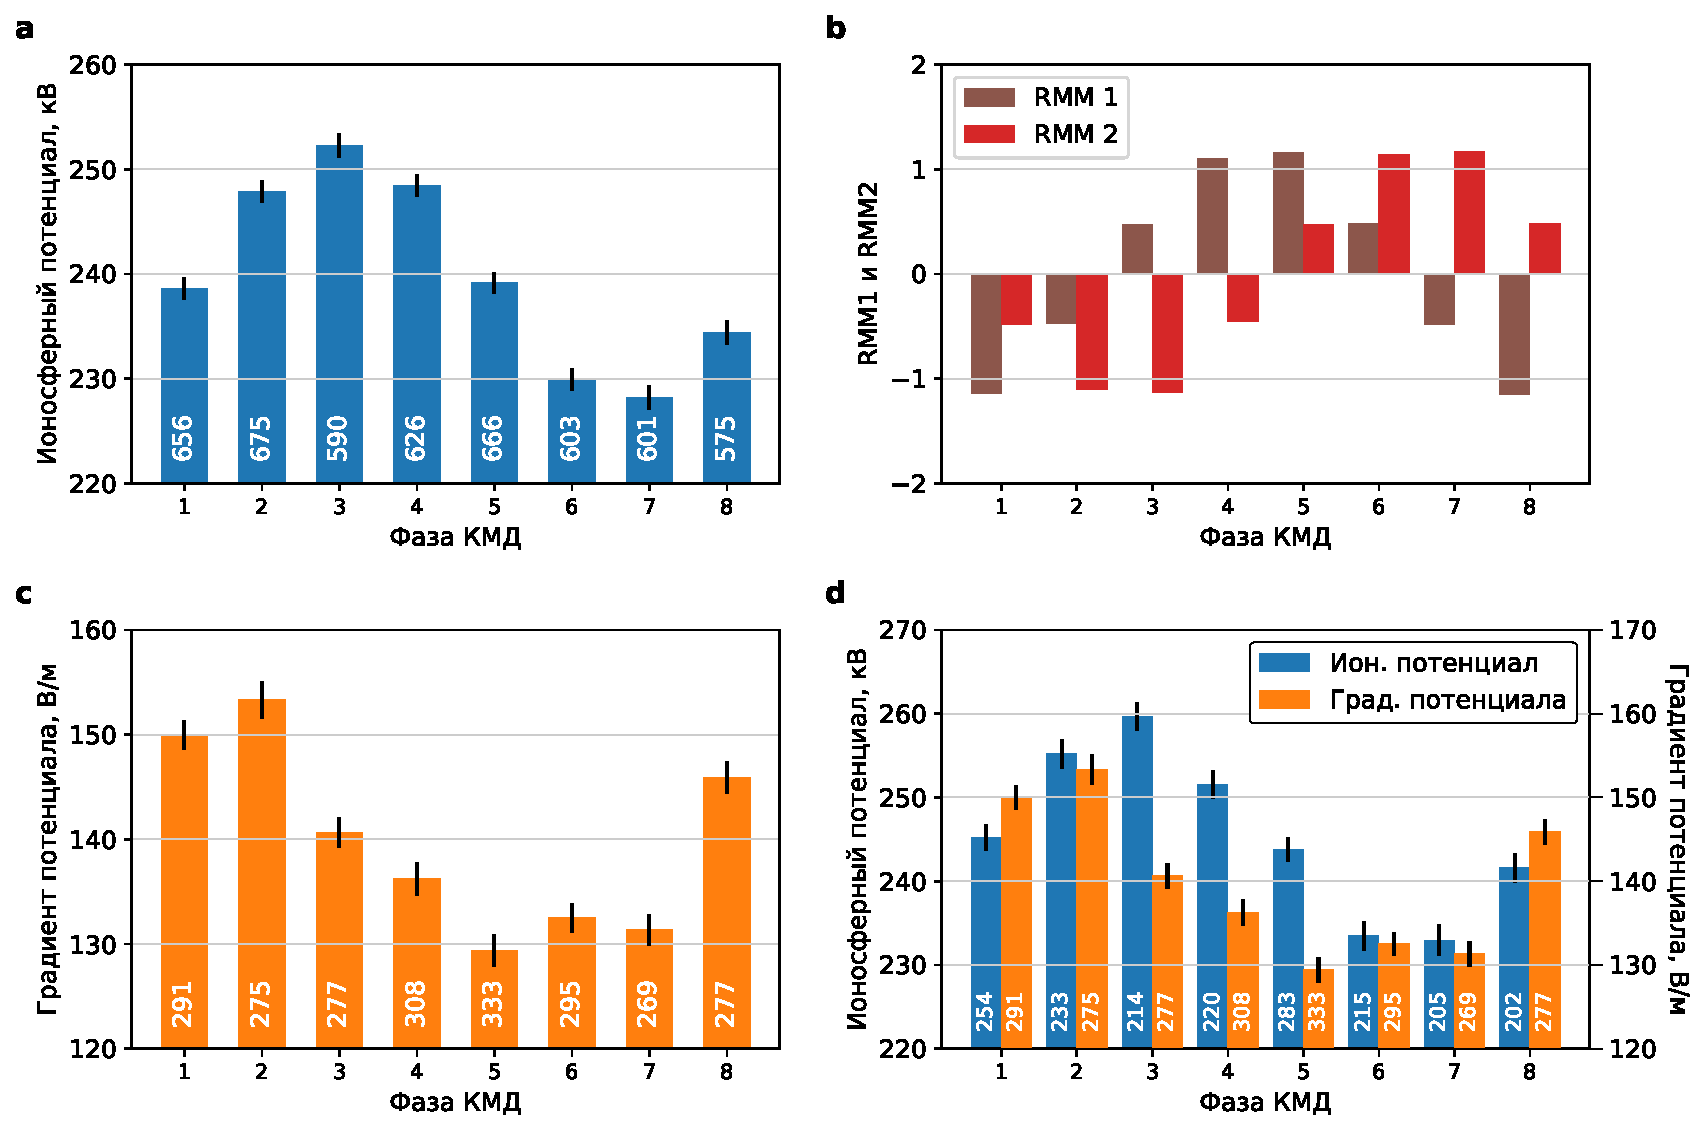
\includegraphics[width=\textwidth]{figures/variations.pdf}
    \caption{(a): Средние значения моделируемого ИП за каждую из фаз КМД (на основе моделирования за 1980--2020). (b): Средние значения компонент индекса RMM за каждую из фаз КМД на основе данных за 1980--2020. (c): Средние значения ГП, измеренного в хорошую погоду на станции Восток, для каждой из фаз КМД (на основе измерений в течение 2006--2020). (d): Сравнение значений ГП, показанных на рисунке (c) со значениями моделируемого ИП за тот же временной интервал (2006--2020). Черные штрихи на столбцах на рисунках (a), (c) и (d) обозначают отклонение в одну стандартную ошибку, а числа в столбцах на тех же рисунках указывают количество дней моделирования или измерений в хорошую погоду, которые пришлись на каждую из фаз КМД.}
    \label{fig:variations}
\end{figure}

Рис. \ref{fig:variations}{b} демонстрирует средние значения RMM1 и RMM2 в различные фазы КМД (на основе данных за 1980--2020). Такие вариации хорошо приближаются синусоидами, ведь фазы КМД возможно определять с помощью полярного угла на плоскости (RMM1, RMM2) (см. рис. \ref{fig:wh04_fig7}), который задается как $\arctg(\mathrm{RMM2}/\mathrm{RMM1})$. Вариации RMM1 и RMM2 имеют схожие амплитуды и сдвинуты друг относительно друга на четверть периода, что отражает тот факт, что усредненная по многим циклам КМД траектория состояния КМД на плоскости (RMM1, RMM2) близка к окружности.

Из сравнения рис. \ref{fig:variations}{b} и \ref{fig:variations}{a} можно заключить, что зависимость ИП от фазы КМД во многом повторяет зависимость величины RMM2, взятой с обратным знаком, от фазы КМД. Точнее, между этими вариациями есть сильная отрицательная корреляция с коэффициентом корреляции $r=-0.93$. В то же время коэффициент корреляции ИП с RMM1 составляет лишь $r=0.33$.

Рассматривается $N = 8$ фаз КМД. Можно оценить значимость наблюдаемой корреляции, используя двухвыборочный t-критерий Стьюдента для независимых выборок с $N - 2 = 6$ степенями свободы. Если даны две независимые выборки размера $N$, а $r$~---~коэффициент корреляции между ними, то величина
\begin{equation}
 	q = \dfrac{r\sqrt{N-2}}{\sqrt{1-r^2}}
\end{equation}
подчиняется распределению Стьюдента. На уровне значимости 1\% гипотеза о том, что две выборки независимы, отвергается, если $q\ge3.71$ или $\abs{r}\ge0.83$. Из данного критерия следует, что отрицательная корреляция между ИП и RMM2 ($r=-0.93$) статистически значима на уровне значимости 1\%, однако связь между ИП и RMM1 ($r=0.33$) не значима.

Если рассматривать данный вопрос более широко, то можно учесть двумерность индекса RMM, что позволяет вместо RMM1 и RMM2 рассматривать проекцию индекса RMM на любое направление в плоскости (RMM1, RMM2), то есть можно оперировать с величиной 
\begin{equation}\label{rmm_direction}
	\mathrm{RMM1}\cdot \cos\phi + \mathrm{RMM2}\cdot \sin\phi,
\end{equation}
где $\phi$~---~полярный угол на плоскости (RMM1, RMM2) (отсчитывается от положительного направления RMM1). Коэффициент корреляции между величиной (\ref{rmm_direction}) и ИП зависит от полярного угла $\phi$ так, как показано на рис. \ref{fig:r} (голубая кривая), и достигает своего максимального значения ($r=0.99$) при $\phi=290^\circ$; на рис. \ref{fig:rmm_diagram} это направление обозначено голубой пунктирной линией. Таким образом, можно утверждать, что значения ИП, будучи усреднены по фазам КМД, крайне хорошо коррелируют с циклом КМД.

\begin{figure}[htbp]
	\centering
	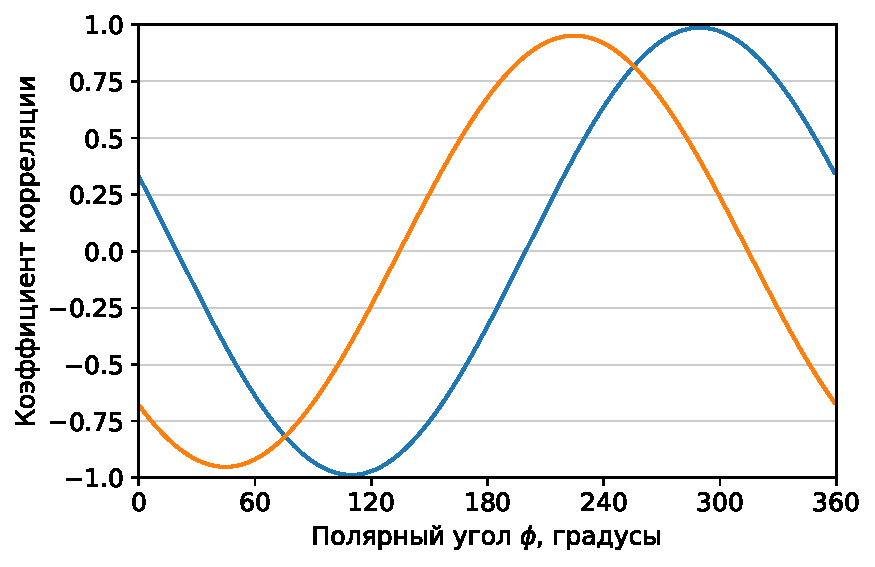
\includegraphics[width=0.6\textwidth]{figures/r.pdf}
	\caption{Коэффициент корреляции между величиной (\ref{rmm_direction}) и ИП (голубая линия), а также между величиной (\ref{rmm_direction}) и ГП (оранжевая линия) в зависимости от полярного угла $\phi$.}
	\label{fig:r}
\end{figure}

Стоит заметить, что направление в сторону отрицательных значений RMM2 соответствует полярному углу $\phi=270^\circ$, что близко к $\phi=290^\circ$, а направление в сторону положительных значений RMM1 соответствует $\phi=0^\circ$, что почти перпендикулярно к направлению $\phi=290^\circ$. Это согласуется с приведенными выше результатами, согласно которым ИП негативно коррелирует с RMM2, но не коррелирует с RMM1.

    \subsection{ЭФФЕКТЫ КМД В РЕЗУЛЬТАТАХ ИЗМЕРЕНИЙ ЭЛЕКТРИЧЕСКОГО ПОЛЯ}

Было показано, что моделируемый ИП имеет синусоидальную вариацию по фазам КМД. Теперь следует исследовать на наличие подобного эффекта результаты измерений ГП на антарктической станции Восток, которые проводились в 2006--2020 (см. раздел \ref{sec:vostok}).

Средние значения ГП, измеренного в хорошую погоду на станции Восток, отвечающие различным фазам КМД продемонстрированы на рис. \ref{fig:variations}{c}. Снова заметна синусоидальная кривая, но менее гладкая, чем та, что получалась для ИП (см. рис. \ref{fig:variations}{a}); вариация ГП имеет максимум в фазе~2 и минимум около фаз 5--7. Точнее, вариация ГП имеет 2 локальных минимума~---~один в фазе~5 и один в фазе~7, которые разделены малым локальным максимумом в фазе~6; однако, так как значения ГП в фазах 5--7 близки, то далее минимумы в фазе~5 и фазе~7 будут пониматься как один минимум.

Если сравнивать динамику моделируемого ИП за 1980--2020 (см. рис. \ref{fig:variations}{a}) и измеренного в хорошую погоду на станции Восток ГП за 2006--2020 (см. рис. \ref{fig:variations}{c}), то можно заметить разницу между двумя такими вариациями. Чтобы сравнение ИП и ГП стало корректным, следует рассматривать значения ГП и значения ИП, усреднённые за одинаковый временной период 2006--2020, что сделано на рис. \ref{fig:variations}{d}. Коэффициент корреляции между двумя вариациями составляет $r=0.50$ (чего не достаточно для статистической значимости на уровне 1\%), но между вариациями присутствует фазовый сдвиг на восьмую часть периода (т.е. на 1 фазу КМД). Если сдвинуть вариацию ГП на 1 фазу вправо, то коэффициент корреляции возрастёт и составит $r=0.90$, чего хватает для статистической значимости на уровне 1\%.

Кроме того, интересно сравнить ГП за дни хорошей погоды с компонентами индекса RMM. Коэффициент корреляции между ГП и RMM1 равен $r=-0.68$, а между ГП и RMM2 коэффициент корреляции составляет $r=-0.67$; ГП одинаковым образом негативно коррелирует с RMM1 и RMM2. Для статистической значимости на уровне 1\% (для чего требуется $\abs{r}\ge0.83$) коэффициенты корреляции слишком малы.

Если рассматривать линейную комбинацию компонент индекса RMM (\ref{rmm_direction}), то коэффициент корреляции между такой линейной комбинацией и ГП, измеренного в дни хорошей погоды, имеет максимальное значение $r=0.95$, что достигается при $\phi=225^\circ$ (см. рис. \ref{fig:r}); такое направление отмечено на рис. \ref{fig:rmm_diagram} оранжевой штрихованной линией. Следует заметить, что такое направление совпадает с биссектрисой третьей четверти фазовой плоскости индекса RMM, что хорошо соотносится с ранними замечаниями о том, что ГП примерно одинаково негативно коррелирует с RMM1 и RMM2. Кроме того, следует отметить, что оптимальное направление для ГП $\phi=225^\circ$ отличается от найденного для моделируемого ИП ($\phi=90^\circ$) на 65\textdegree, что соответствует примерно 1.5 фазам КМД.

Таким образом, было установлено, что как значения ИП, так и значения ГП (усреднённые по фазам КМД) коррелируют с циклом КМД на статистически значимом уровне в 1\%, но их вариации по фазам КМД имеют фазовый сдвиг друг относительно друга. Штрихи на рис. \ref{fig:variations} обозначают плюс и минус одну стандартную ошибку (что равно стандартному отклонению среднего). Из рис. \ref{fig:variations}{d} видно, что несогласие между формами двух вариаций не могут быть объяснены только лишь статистическими ошибками. Другие возможные объяснения различия вариаций заключаются в неточности используемой параметризации ИП, в воздействии локальных эффектов на результаты измерений ГП и в воздействии солнечной активности. Эти вопросы будут обсуждены ниже в разделе ? .
    \Subsection{Детальное обсуждение и объяснение физических механизмов}\label{subsec:2-6}

Так как была обнаружена связь КМД с ИП в том числе и в результатах моделирования ГЭЦ, то возможно проанализировать найденную связь более детально, используя данные вкладов одиночных столбцов модели. В данном подразделе будет предпринята попытка разложить вариацию ИП на простые колебания, чтобы понять физический механизм, лежащий за наблюдаемым эффектом.
    \subsection{НЕКОТОРЫЕ ЗАМЕЧАНИЯ}

В данном разделе будут даны некоторые замечания и описаны возможные объяснения тех мест описанного выше исследования, которые могли остаться не понятны.

\subsubsection{ВОСПРОИЗВОДИМОСТЬ РЕЗУЛЬТАТОВ}

В разделах \ref{sec:eff_mjo_gec}, \ref{sec:mjo_pg} и \ref{sec:futher_analysis} было показано, что КМД воздействует на интенсивность ГЭЦ постоянного тока. Было установлено, что моделируемый ИП и ГП, измеряемые в дни хорошей погоды на станции Восток, дают близкие к синусоидальным вариации по фазам КМД и имеют статистически значимую связь с индексами, характеризующими КМД.

Важно заметить, что вариации параметров ГЭЦ, представленные на рис. \ref{fig:variations}{a} и  \ref{fig:variations}{c}, не случайны. Аналогично рис. \ref{fig:variations}{a}, рис. \ref{fig:ip_pg_variation_partial}{a}--\ref{fig:ip_pg_variation_partial}{d} демонстрируют вариацию ИП по фазам КМД при усреднении не за весь 41 год моделирования, а при усреднении по различным десятилетиям. Хотя среднее значение ИП в каждое из десятилетий отличается от других, это не мешает наблюдать характерную близкую к синусоидальной вариацию ИП по фазам КМД в каждое из десятилетий.

\begin{figure}[htbp]
    \centering
    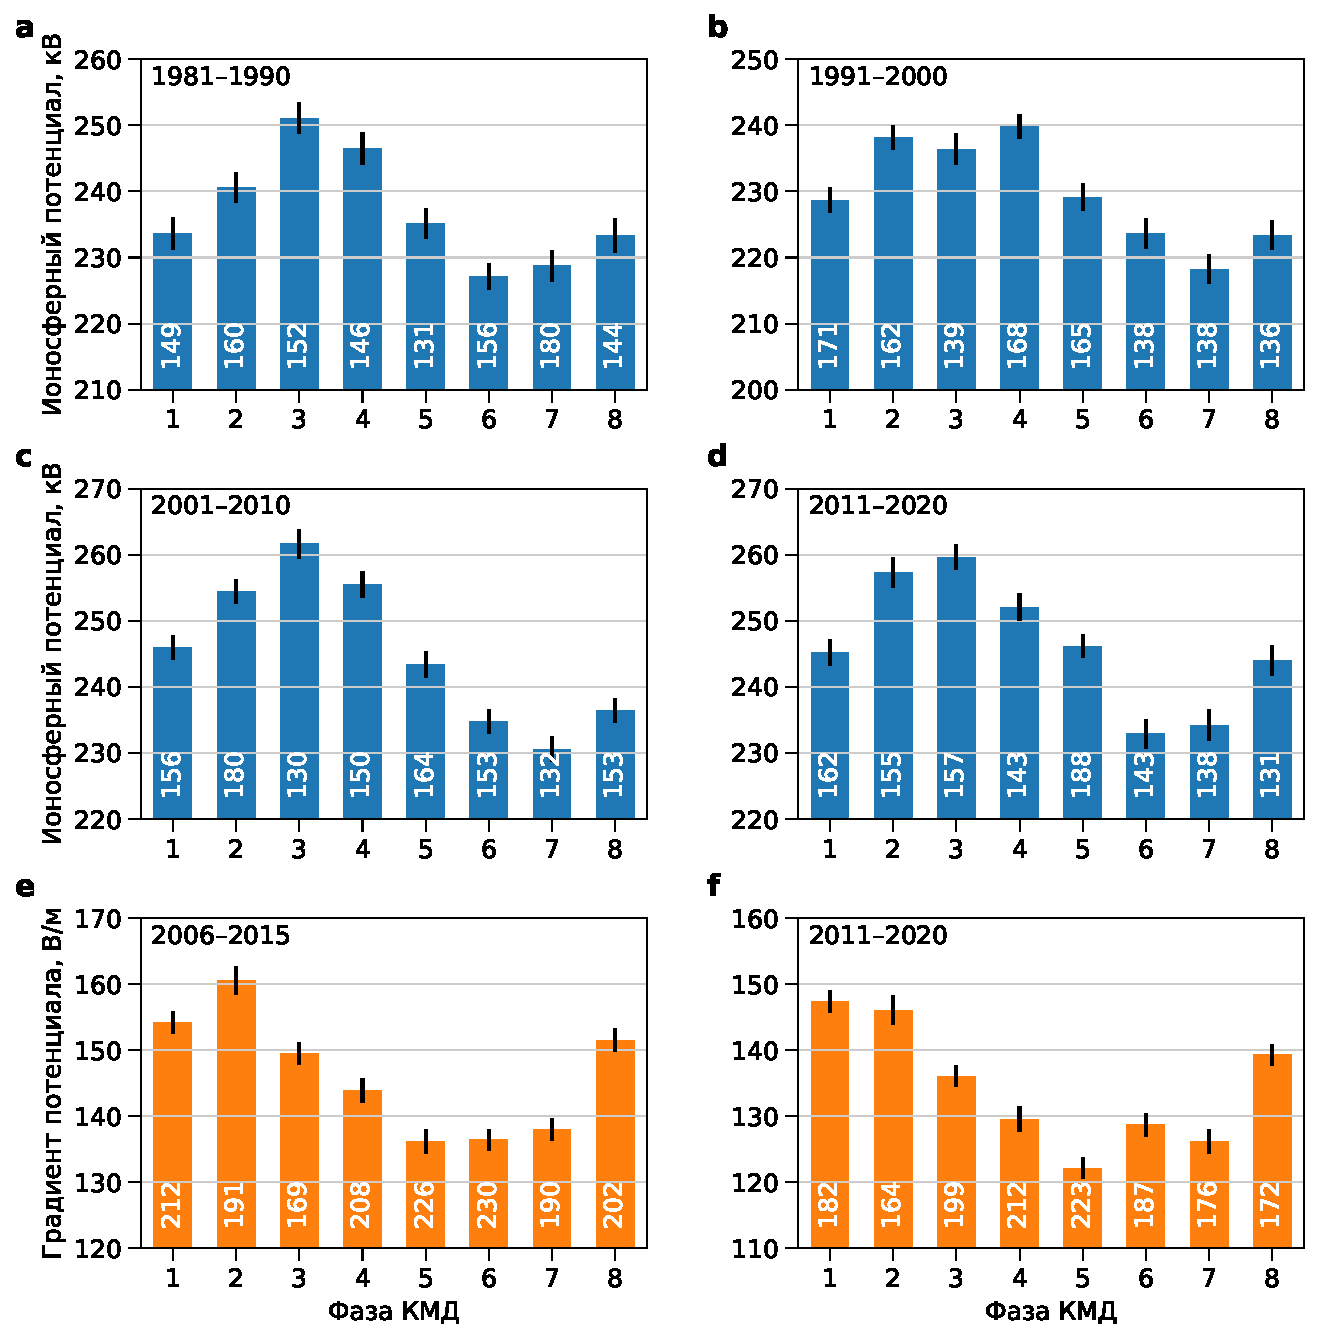
\includegraphics[width=\textwidth]{figures/ip_pg_variation_partial.pdf}
    \caption{(a)--(d): Усредненные значения ИП за каждую из фаз КМД на основе моделирования за 41 года (с 1 января 1980 года по 29 декабря 2020), первые четыре десятилетия рассмотрены раздельно. (e), (f): Средние значения ГП за дни хорошей погоды со станции Восток за каждую из фаз КМД на основе измерений в течение 2006--2015 и 2011--2020. Числа в столбцах означают, какое количество дней соответствует каждой из фаз КМД; черные штрихи на столбцах обозначают отклонение в одну стандартную ошибку.}
    \label{fig:ip_pg_variation_partial}
\end{figure}

Рис. \ref{fig:ip_pg_variation_partial}{e} и \ref{fig:ip_pg_variation_partial}{f} являются аналогами рис. \ref{fig:variations}{c} для двух перекрывающихся десятилетий 2006--2015 и 2011--2020. Из сравнения рис. \ref{fig:ip_pg_variation_partial}{e}, \ref{fig:ip_pg_variation_partial}{f} и \ref{fig:variations}{c}, видно, что форма вариации ГП по фазам КМД в целом не меняется (в случае 2011--2020 максимум сдвигается в первую фазу, однако значения ГП в первую и вторую фазу имеют перекрывающиеся интервалы стандартных ошибок), следовательно имеет универсальный характер.

Таким образом, получается выделить в ГЭЦ паттерны, явно связанные с КМД. Кроме исследований связей КМД с резонансами Шумана \cite{Anyamba_et_al_2000, Beggan_Musur_2019}, в литературе отсутствуют какие-либо исследования о воздействии КМД на электрическое окружение Земли. Учитывая недавно обнаруженную связь ЭНЮК с ГЭЦ постоянного тока \cite{Harrison_et_al_2011, Slyunyaev_et_al_2021a, Slyunyaev_et_al_2021b, Slyunyaev_et_al_2021c}, результаты данной работы позволяют подчеркнуть, что ГЭЦ является важной частью земной системы и отражает климатическую изменчивость, происходящую на различных временных масштабах. Стоит заметить, что параметры ГЭЦ как в случае с ЭНЮК, так и в случае с КМД требуют усреднения по многим событиям для обнаружения связей с рассматриваемыми климатическими модами.

\subsubsection{ЗАМЕЧАНИЯ ОТНОСИТЕЛЬНО ЭОФ-АНАЛИЗА}

Моделирование позволяет не только обнаружить эффект КМД в ГЭЦ, но и исследовать физический механизм, обеспечивающий наблюдаемый эффект. С данной целью ко вкладам экваториального региона, усредненным вдоль меридианов, был применен ЭОФ-анализ, который широко используется при исследовании КМД. ЭОФ задают базис пространственных паттернов, выбираемых таким образом, чтобы временные коэффициенты (ГК) разложения по первым нескольким из них, объясняли наибольшую возможную часть дисперсии. Это позволяет перейти от сложного исходного процесса к суперпозиции нескольких простых процессов.

Указанные в легенде рис. \ref{fig:eofs_and_pcs}{b} и \ref{fig:eofs_and_pcs}{e} числа обозначают объясняемую дисперсию каждой ЭОФ; если просуммировать эти числа, то окажется, что первые три ЭОФ объясняют лишь около 21\% исходной дисперсии. Не стоит удивляться столь малому проценту объясняемой дисперсии: дело в том, что вклады в ИП содержат изменчивость на многих масштабах, и большая часть этой изменчивости не имеет отношение к КМД. Данный факт можно продемонстрировать наглядным примером. На рис. \ref{fig:eofs_and_pcs}{d} изображен вклад в вариацию ИП от ЭОФ3$^\prime$. Видно, что вклад от данной ЭОФ в вариацию ИП по фазам КМД почти нулевой, хотя объясняемая дисперсия для ЭОФ3$^\prime$ составляет около 6\% --- значение, близкое к величинам объясняемой дисперсии ЭОФ1 (около 8\%) и ЭОФ2$^\prime$ (около 6\%), которые являются базовыми.

\subsubsection{ФАЗОВЫЙ СДВИГ МЕЖДУ ИП И ГП}
\label{sec:phase_shift}

Как показано в разделах \ref{sec:eff_mjo_gec} и \ref{sec:mjo_pg}, моделируемый ИП и измеряемый на станции Восток ГП за дни хорошей погоды имеют статистически значимую связь с циклом КМД. В то же время имеет место фазовый сдвиг между двумя такими параметрами ГЭЦ: ИП достигает максимального значения в третьей фазе КМД (см. рис. \ref{fig:variations}{a}) и имеет наибольший коэффициент корреляции с \eqref{rmm_direction} при $\phi = 290\text{\textdegree}$ (см. рис. \ref{fig:rmm_diagram}), а ГП достигает максимального значения во второй фазе (см. рис. \ref{fig:variations}{c}) и наиболее коррелирован с \eqref{rmm_direction} при $\phi = 225\text{\textdegree}$ (см. рис. \ref{fig:rmm_diagram}). 

Из теоретических соображений следует, что приповерхностный ГП в хорошую погоду связан с ИП соотношением \eqref{eq:pg_ip}. Такая формула напрямую отражает глобальный характер ГЭЦ: токи, обусловленные разделением зарядов в грозовых облаках и ESC по всей Земле, поднимаются вверх, обеспечивая вместе ИП, а затем стекают от ионосферы вниз к поверхности Земли через области хорошей погоды. Если пренебречь вариациями проводимости, то в хорошую погоду ГП прямо пропорционален ИП и отражает его динамику, как видно из \eqref{eq:pg_ip}. Однако в случае с КМД между измеряемым на станции Восток ГП и моделируемым ИП имеется фазовый сдвиг в примерно полторы фазы КМД, что не укладывается в рамки вышеописанного подхода. Ниже будут рассмотрены несколько наиболее вероятных причин, которые могли бы привести к наличию наблюдаемого сдвига.

Во-первых, к такому сдвигу могли привести ошибки параметризации ИП \eqref{eq:ip}. Возможно, вклады Морского континента и Восточной части Тихого океана в ИП переоцениваются рассматриваемой параметризацией \cite{Ilin_et_al_2020}. Учитывая тот факт, что ЭОФ1 описывает вклады в ИП в основном от Морского континента (см. рис. \ref{fig:eofs_and_pcs}{e}), такая переоценка могла бы привести к увеличению амплитуды изменчивости той части ИП, которая отвечает ЭОФ1. Если данная гипотеза верна, то при учете ошибки параметризации следует ожидать, что вариация ИП по фазам КМД в значительной степени будет складываться из вкладов, отвечающих ЭОФ2$^\prime$, что сдвинет максимум вариации ИП в сторону второй фазы.

Во-вторых, возможно, что наблюдаемое различие между ГП и ИП было вызвано различными факторами, влияющими на измерения ГП. Одним из таких факторов, влияющих на измерения ГП в Антарктике, является солнечная активность \cite{Burns_et_al_2017}. Солнечная активность влияет на процессы ионизации в атмосфере и тем самым возмущает проводимость воздуха (кроме того, солнечная активность может модулировать интенсивность источников ГЭЦ, но по данному вопросу ещё нет конечного понимания в мировом научном сообществе). Наиболее близкой к временным масштабам КМД (20--90 суток) является 27-дневный солнечный цикл, связанный со вращением Солнца вокруг своей оси. Естественно полагать, что 27-дневный солнечный цикл будет влиять на ГП на масштабах КМД. Следует отметить, что влияние солнечной активности на проводимость воздуха в рассматриваемой параметризации ИП \eqref{eq:ip} учтено не был, отсюда может проистекать наблюдаемое различие между вариациями ГП и ИП по фазам КМД.

% описать что вообще не так
% описать как текут токи, привести формулу, связывающую ГП в хорошую погоду и ИП пропорциональным соотнесением
% Рассмотреть вариант воздействия например ветра на измерения гп, для этого надо взять ветер на какой-нибудь низкой высоте, построить скаттер-плот мб, а самое главное посмотреть как коррелирует какой-нибудь параметр ветра с кмд или нет (типа главная гипотеза, которую ты здесь хочешь проверить --- дальняя связь КМД с ветром на станции восток дает фазовый сдвиг, хотя мб лучше вот как сделать: связан ли вообще этот ветер хоть как=то с кмд, если нет, то фуфло у тебя, а не гипотеза)
    
    % ?? описание используемой модели ГЭЦ %
    % описание измерений ГП на станции Восток %
    % эффекты КМД в ГЭЦ, обнаруженные при моделировании
    % Большой и подробный раздел про объяснение вариации ИП по фазам КМД
    % Эффекты КМД в измерениях ГП
    % обсуждение причин несостыковок
    
    \newpage
     \section{ЗАКЛЮЧЕНИЕ}

В рамках первой части настоящей работы была программно реализована столбчатая модель глобальной электрической цепи (ГЭЦ). Источники в модели задавались путем выделения столбцов воздуха, характеризуемых глубокой конвекцией, по критерию, основанному на значении доступной конвективной потенциальной энергии; площадь области смешанной фазы в данном столбце оценивалась через отношение величины осадков к величине запасенной влаги в столбе воздуха. \textbf{При помощи созданной модели ГЭЦ можно анализировать задачи, связанные с крупномасштабными возмущениями проводимости воздуха.}

% Была произведена серия расчетов ионосферного потенциала (ИП). Каждая серия расчетов производилась с различной параметризацией проводимости атмосферы: с простой экспоненциальной проводимостью и с более сложной параметризацией, учитывающей влияние солнечной активности, при различных уровнях солнечной активности. В результате каждой серии расчетов был получен 24-часовой набор данных ИП для каждого третьего дня 2016 года.

Разработанная модель ГЭЦ позволила получить кривую суточной вариации ионосферного потенциала (ИП), которая близка к экспериментальной кривой Карнеги, что подтверждает корректность работы созданной реализации столбчатой модели ГЭЦ. Анализ результатов расчетов ИП показал, что \textbf{форма кривой суточной вариации ИП, которая получается при моделировании с экспоненциальной проводимостью, совпадает с кривой, которая получается при моделировании с учетом более реалистичной проводимости.} Кроме того, удалось установить, что \textbf{учет более реалистичной проводимости приводит к повышению ИП примерно на 10~кВ в фазу максимума солнечной активности и к понижению примерно на те же 10~кВ в фазу минимума солнечной активности} относительно средних значений ИП.

Во второй части работы было обнаружено, что \textbf{как моделируемый ИП, так и измеряемый на полярной станции Восток приповерхностный градиент потенциала (ГП) электрического поля имеют синусоидальные вариации по фазам колебания Мад\-де\-на--Джу\-ли\-ана (КМД);} такие вариации имеют статистически значимые корреляции с выбираемыми соответствующим образом проекциями двумерного индекса RMM (Real-time Multivariate MJO index), характеризующего КМД.

Более глубокое исследование с использованием эмпирических ортогональных функций, вычисляемых на основе вкладов в ИП, позволило выделить во вкладах паттерны, близкие к тем паттернам конвекции, которые характерны для КМД. \textbf{Большая часть изменчивости ИП на масштабах КМД объясняется двумя базовыми колебаниями конвекции, одно из которых происходит над Юго-Восточной Азией, а другое --- над Индийским океаном.} Такие колебания имеют естественную связь с компонентами индекса RMM. Кроме того, на основе вкладов в ИП, которые имеют ясный физический смысл, можно даже выделить новый индекс КМД.

Несмотря на небольшое расхождение по фазе между вариациями \textbf{ИП и ГП} на масштабах КМД (вероятно, связанное с недостатками моделирования ИП и с влиянием локальных эффектов на результаты измерений ГП), обе величины \textbf{показывают высокую и статистически значимую корреляцию с циклом КМД;} вместе с более ранними результатами о связи ЭНЮК и ГЭЦ \cite{Slyunyaev_et_al_2021a, Slyunyaev_et_al_2021b, Harrison_et_al_2011, Slyunyaev_et_al_2021c, Lavigne_et_al_2017} это позволяет говорить об отражении различных климатических мод в атмосферном электричестве.

%Было обнаружено расхождение результатов моделирования ИП с результатами измерений ГП: существует фазовый сдвиг между вариациями ИП и ГП на масштабах КМД. Данный сдвиг составляет примерно полторы фазы КМД и может быть списан на ошибки моделирования ИП и на влияние локальных эффектов на измерения ГП. Однако точной причины наблюдаемого расхождения пока не установлено. Первым шагом на пути к пониманию причин наличия расхождения может стать долгосрочное моделирование ГЭЦ с более реалистичной проводимостью, учитывающей влияние солнечной активности. Для этих целей может быть использована столбчатая модель ГЭЦ, разработанная в первой части работы.
    % ЗАКЛЮЧЕНИЕ

    \newpage
    \addcontentsline{toc}{section}{СПИСОК ЛИТЕРАТУРЫ}
    \bibliographystyle{unsrt}
    %\bibliography{inc/references}
    \begin{thebibliography}{10}

\bibitem{Williams_Mareev_2014}
E.~Williams and E.~Mareev.
\newblock Recent progress on the global electrical circuit.
\newblock {\em Atmos.\ Res.}, 135--136:208--227, 2014.

\bibitem{Rycroft_et_al_2008}
M.~J. Rycroft, R.~G. Harrison, K.~A. Nicoll, and E.~A. Mareev.
\newblock An overview of {E}arth’s global electric circuit and atmospheric
  conductivity.
\newblock {\em Space Sci.\ Rev.}, 137(1--4):83--105, 2008.

\bibitem{Williams_2009}
E.~R. Williams.
\newblock The global electrical circuit: A review.
\newblock {\em Atmos.\ Res.}, 91(2--4):140--152, 2009.

\bibitem{Markson_2007}
R.~Markson.
\newblock The global circuit intensity: Its measurement and variation over the
  last 50 years.
\newblock {\em Bull.\ Amer.\ Meteor.\ Soc.}, 88(2):223--241, 2007.

\bibitem{Ilin_et_al_2020}
N.~V. Ilin, N.~N. Slyunyaev, and E.~A. Mareev.
\newblock Toward a realistic representation of global electric circuit
  generators in models of atmospheric dynamics.
\newblock {\em J.\ Geophys.\ Res.\ Atmos.}, 125(6):e2019JD032130, 2020.

\bibitem{Slyunyaev_et_al_2015}
N.~N. Slyunyaev, E.~A. Mareev, and A.~A. Zhidkov.
\newblock On the variation of the ionospheric potential due to large-scale
  radioactivity enhancement and solar activity.
\newblock {\em Journal of Geophysical Research: Space Physics},
  120(8):7060--7082, 2015.

\bibitem{Madden_Julian_1994}
R.~A. Madden and P.~R. Julian.
\newblock Observations of the 40–50-day tropical oscillation—{A} review.
\newblock {\em Mon.\ Wea.\ Rev.}, 122(5):814--837, 1994.

\bibitem{Zhang_2005}
C.~Zhang.
\newblock {M}adden-{J}ulian {O}scillation.
\newblock {\em Rev.\ Geophys.}, 43(2):RG2003, 2005.

\bibitem{Zhang_et_al_2020}
C.~Zhang, {\'A}.~F. Adames, B.~Khouider, B.~Wang, and D.~Yang.
\newblock Four theories of the {M}adden-{J}ulian {O}scillation.
\newblock {\em Rev.\ Geophys.}, 58(3):e2019RG000685, 2020.

\bibitem{Anyamba_et_al_2000}
E.~Anyamba, E.~Williams, J.~Susskind, A.~Fraser-Smith, and M.~Fullekrug.
\newblock The manifestation of the {M}adden–{J}ulian oscillation in global
  deep convection and in the {S}chumann resonance intensity.
\newblock {\em J.\ Atmos.\ Sci.}, 57(8):1029--1044, 2000.

\bibitem{Beggan_Musur_2019}
C.~D. Beggan and M.~A. Musur.
\newblock Is the {M}adden–{J}ulian {O}scillation reliably detectable in
  {S}chumann {R}esonances?
\newblock {\em J.\ Atmos.\ Sol.\ Terr.\ Phys.}, 190:108--116, 2019.

\bibitem{Slyunyaev_et_al_2021a}
N.~N. Slyunyaev, A.~V. Frank-Kamenetsky, N.~V. Ilin, F.~G. Sarafanov, M.~V.
  Shatalina, E.~A. Mareev, and C.~G. Price.
\newblock Electric field measurements in the {A}ntarctic reveal patterns
  related to the {E}l {N}iño—{S}outhern {O}scillation.
\newblock {\em Geophys.\ Res.\ Lett.}, 48(21):e2021GL095389, 2021.

\bibitem{Slyunyaev_et_al_2021b}
N.~N. Slyunyaev, N.~V. Ilin, E.~A. Mareev, and C.~G. Price.
\newblock The global electric circuit land–ocean response to the {E}l
  {N}iño—{S}outhern {O}scillation.
\newblock {\em Atmos.\ Res.}, 260:105626, 2021.

\bibitem{Harrison_et_al_2011}
R.~G. Harrison, M.~Joshi, and K.~Pascoe.
\newblock Inferring convective responses to {E}l {N}iño with atmospheric
  electricity measurements at {S}hetland.
\newblock {\em Environ.\ Res.\ Lett.}, 6(4):044028, 2011.

\bibitem{Slyunyaev_et_al_2021c}
N.~N. Slyunyaev, N.~V. Ilin, E.~A. Mareev, and C.~G. Price.
\newblock A new link between {E}l {N}iño—{S}outhern {O}scillation and
  atmospheric electricity.
\newblock {\em Environ.\ Res.\ Lett.}, 16(4):044025, 2021.

\bibitem{Mareev_2010}
Е.~А. Мареев.
\newblock Достижения и перспективы
  исследований глобальной электрической
  цепи.
\newblock {\em Усп. физ. наук}, 180(5):527--534, 2010.

\bibitem{Kalinin_et_al_2014}
А.~В. Калинин, Н.~Н. Слюняев, Е.~А. Мареев и
  А.~А. Жидков.
\newblock Стационарные и нестационарные модели
  глобальной электрической цепи:
  корректность, аналитические соотношения,
  численная реализация.
\newblock {\em Известия Российской Академии Наук.
  Физика Атмосферы и Океана}, 50(3):355--364, 2014.

\bibitem{Mareev_Volodin_2014}
E.~A. Mareev and E.~M. Volodin.
\newblock Variation of the global electric circuit and ionospheric potential in
  a general circulation model.
\newblock {\em Geophys.\ Res.\ Lett.}, 41(24):9009--9016, 2014.

\bibitem{Harrison_2012}
R.~Harrison.
\newblock The {C}arnegie curve.
\newblock {\em Surveys in Geophysics}, 34:209--232, 03 2012.

\bibitem{Madden_Julian_1972}
R.~A. Madden and P.~R. Julian.
\newblock Description of global-scale circulation cells in the tropics with a
  40–50 day period.
\newblock {\em J.\ Atmos.\ Sci.}, 29(6):1109--1123, 1972.

\bibitem{Wheeler_Hendon_2004}
M.~C. Wheeler and H.~H. Hendon.
\newblock An all-season real-time multivariate {MJO} index: Development of an
  index for monitoring and prediction.
\newblock {\em Mon.\ Wea.\ Rev.}, 132(8):1917--1932, 2004.

\bibitem{Wang_et_al_2018}
Feiyang Wang, Wenshou Tian, Fei Xie, Jiankai Zhang, and Yuanyuan Han.
\newblock Effect of {M}adden–{J}ulian oscillation occurrence frequency on the
  interannual variability of northern hemisphere stratospheric wave activity in
  winter.
\newblock {\em Journal of Climate}, 31:5031--5049, 2018.

\bibitem{Burns_et_al_2012}
G.~B. Burns, B.~A. Tinsley, A.~V. Frank‐Kamenetsky, O.~A. Troshichev,
  W.~J.~R. French, and A.~R. Klekociuk.
\newblock Monthly diurnal global atmospheric circuit estimates derived from
  {V}ostok electric field measurements adjusted for local meteorological and
  solar wind influences.
\newblock {\em J.\ Atmos.\ Sci.}, 69(6):2061--2082, 2012.

\bibitem{Burns_et_al_2017}
G.~B. Burns, A.~V. Frank-Kamenetsky, B.~A. Tinsley, W.~J. French, P.~Grigioni,
  G.~Camporeale, and E.~A. Bering.
\newblock Atmospheric global circuit variations from {V}ostok and {C}oncordia
  electric field measurements.
\newblock {\em J.\ Atmos.\ Sci.}, 74(3):783--800, 2017.

\bibitem{Knutson_Weickmann_1987}
T.~R. Knutson and K.~M. Weickmann.
\newblock 30–60 day atmospheric oscillations: Composite life cycles of
  convection and circulation anomalies.
\newblock {\em Mon.\ Wea.\ Rev.}, 115(7):1407--1436, 1987.

\bibitem{Slingo_et_al_1999}
J.~M. Slingo, D.~P. Rowell, K.~R. Sperber, and F.~Nortley.
\newblock On the predictability of the interannual behaviour of the
  {M}adden–{J}ulian {O}scillation and its relationship with {E}l {N}iño.
\newblock {\em Quart.\ J.\ Roy.\ Meteor.\ Soc.}, 125(554):583--609, 1999.

\bibitem{Lo_Hendon_2000}
F.~Lo and H.~H. Hendon.
\newblock Empirical extended-range prediction of the {M}adden–{J}ulian
  oscillation.
\newblock {\em Mon.\ Wea.\ Rev.}, 128(7):2528--2543, 2000.

\bibitem{Matthews_2000}
A.~J. Matthews.
\newblock Propagation mechanisms for the {M}adden-{J}ulian {O}scillation.
\newblock {\em Quart.\ J.\ Roy.\ Meteor.\ Soc.}, 126(569):2637--2651, 2000.

\bibitem{Kessler_2001}
W.~S. Kessler.
\newblock {EOF} representations of the {M}adden–{J}ulian oscillation and its
  connection with {ENSO}.
\newblock {\em J.\ Climate}, 14(13):3055--3061, 2001.

\bibitem{Adlerman_Williams_1996}
E.~J. Adlerman and E.~R. Williams.
\newblock Seasonal variation of the global electrical circuit.
\newblock {\em J.\ Geophys.\ Res.}, 101(D23):29679--29688, 1996.

\bibitem{Zhang_Moore_2015}
Z.~Zhang and J.~C. Moore.
\newblock {\em Mathematical and Physical Fundamentals of Climate Change}.
\newblock Elsevier, Amsterdam, Netherlands, 2015.

\bibitem{Lavigne_et_al_2017}
T.~Lavigne, C.~Liu, W.~Deierling, and D.~Mach.
\newblock Relationship between the global electric circuit and electrified
  cloud parameters at diurnal, seasonal, and interannual timescales.
\newblock {\em J.\ Geophys.\ Res.\ Atmos.}, 122(16):8525--8542, 2017.

\end{thebibliography}

\end{document}